\section{The Ring and Its Linearization}
\label{sec:ring}

We fix a certain exact radial steady state supported in an annulus, which we
call the \textbf{Ring}, and study its linearization, that of the Euler equations
at the Ring plus a point vortex of circulation $2\pi G$ at the origin.

\subsection{The Ring}
\label{sec:ring-def}

\begin{definition}
\label{def:ring}
Put
\[
\begin{gathered}
a_0=-7304210039150669\cdot2^{-54},\qquad d=5764607523034235\cdot2^{-58},\\
\xiL=-4528212286209965\cdot2^{-52},\qquad \xia=-4077852323472915\cdot2^{-52},\\
\xib=\tfrac12,\qquad \xiR=5404319552844595\cdot2^{-53},
\end{gathered}
\]
and $H(x)=(1+e^{-2x})^{-1}$ for $x\in\R$. Fix, once and for all, a function
$\chi\in C_c^\infty(\R)$ with values in $[0,1]$ that is nondecreasing on
$(-\infty,\xia]$, equal to $1$ on $[\xia,\xib]$, nonincreasing on
$[\xib,\infty)$, and supported in $[\xiL,\xiR]$ (such functions exist by
Lemma~\ref{lem:ring-facts}). Put
\[
\begin{gathered}
\prof(\xi)=\chi(\xi)\,H\Big(\frac{\xi-a_0}{d}\Big)H\Big(-\frac{\xi}{d}\Big)\quad(\xi\in\R),\\
\omc(x)=\prof(\log|x|)\quad(x\ne0),\qquad \omc(0)=0,
\end{gathered}
\]
\[
\Rc=e^{\xiR},\qquad \Phi(y)=\omc(\Rc y),\qquad a=e^{\xiL-\xiR},\qquad
\Gone=\tfrac1{50}\Rc^{-2}.
\]
To four significant figures, $a_0\approx-0.4055$, $d\approx0.02000$,
$\xiL\approx-1.005$, $\xia\approx-0.9055$, $\xiR\approx0.6000$,
$\Rc\approx1.822$, $a\approx0.2008$ and $\Gone\approx0.006024$.
We call $\Phi$ \textbf{the ring}. The functions $\omc$ and $\Phi$ describe the
same ring in the variables $x$ and $y$, related by $x=\Rc y$; we say that
$\omc$ is the ring in \textbf{reference units} and $\Phi$ the ring in
\textbf{ring units}. From now on $m=3$, except where an integer $m\ge1$ is
quantified explicitly.
\end{definition}

Figure~\ref{fig:ring} shows the ring, for the function $\chi$ constructed in the
proof of Lemma~\ref{lem:ring-facts}.

\begin{figure}[ht]
\centering
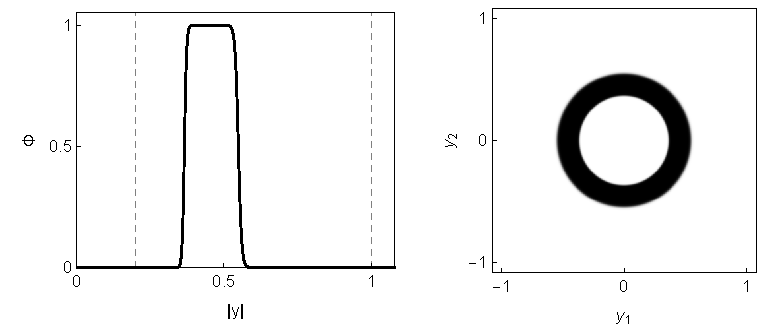
\includegraphics[width=0.85\textwidth]{figures/ring.pdf}
\caption{The ring $\Phi$ of Definition~\ref{def:ring} in ring units, for the
function $\chi$ constructed in the proof of Lemma~\ref{lem:ring-facts}. Left:
the radial profile $\Phi(|y|)$; the dashed lines mark $|y|=a$ and $|y|=1$, between
which $\Phi$ is supported. Right: $\Phi$ on the plane, darker where $\Phi$ is larger
(black on the plateau, where $\Phi$ is close to $1$).
Drawn with Mathematica from the exact formulas; the figure is an illustration and
is not used in any proof.}
\label{fig:ring}
\end{figure}

\begin{lemma}
\label{lem:ring-facts}
A function $\chi$ as in Definition~\ref{def:ring} exists. Moreover
$a_0<0<d$, $\xiL<\xia\le a_0/2\le\xib<\xiR$, $\ell d<1$ for every integer
$1\le\ell\le9$, and $0<a<1$. The function $\omc$ lies in $C_c^\infty(\R^2)$, is
radial, satisfies $0\le\omc<1$, and $\supp\omc\subset\{e^{\xiL}\le|x|\le e^{\xiR}\}$.
Consequently $\Phi\in C_c^\infty(\R^2)$ is radial, $0\le\Phi<1$, $\Phi\not\equiv0$,
and $\supp\Phi\subset\{a\le|y|\le1\}$.
\end{lemma}
\begin{proof}
Let $e(x)=e^{-1/x}$ for $x>0$ and $e(x)=0$ for $x\le0$, and
$S(x)=e(x)/(e(x)+e(1-x))$. Then $S\in C^\infty(\R)$ is nondecreasing, $S=0$ on
$(-\infty,0]$ and $S=1$ on $[1,\infty)$. The function
\[
\chi(\xi)=S\Big(\frac{\xi-\xiL}{\xia-\xiL}\Big)\,S\Big(\frac{\xiR-\xi}{\xiR-\xib}\Big)
\]
is smooth with values in $[0,1]$. Its second factor is $1$ for $\xi\le\xib$ and
its first factor is $1$ for $\xi\ge\xia$; since $\xia\le\xib$, $\chi$ is the
first factor on $(-\infty,\xia]$, $1$ on $[\xia,\xib]$, the second factor on
$[\xib,\infty)$, and $0$ outside $[\xiL,\xiR]$. It has the required properties
once the order of the data is checked.

We compare the data as fractions with a common power of two. The signs of $a_0$
and $d$ are those of their numerators; $4528212286209965>4077852323472915$ gives
$\xiL<\xia$; $a_0/2=-7304210039150669\cdot2^{-55}$ and
$\xia=-32622818587783320\cdot2^{-55}$ give $\xia<a_0/2<0<\xib$; and
$\xib=4503599627370496\cdot2^{-53}<\xiR$. For $\ell d<1$ it suffices to take
$\ell=9$: $9\cdot5764607523034235=\nobreak51881467707308115<2^{58}=\nobreak288230376151711744$.
Since $\xiL<\xiR$, $0<a<1$.

Since $\prof$ is smooth and supported in $[\xiL,\xiR]$, $\omc$ is smooth on
$\R^2\setminus\{0\}$ and vanishes on $B_{e^{\xiL}}$, so $\omc\in C_c^\infty(\R^2)$
with the stated support. Since $0<H<1$ and $0\le\chi\le1$, $0\le\omc<1$. The
statements on $\Phi$ follow from $e^{\xiL}/\Rc=a$, $e^{\xiR}/\Rc=1$, and
$\Phi\not\equiv0$ because ${\prof(\xia)=H((\xia-a_0)/d)H(-\xia/d)>0}$.
\end{proof}

In ring units we use the closed annuli
\[
N=\{\tfrac a2\le|y|\le2\},\qquad N'=\{\tfrac a4\le|y|\le3\};
\]
so $\{a\le|y|\le1\}\subset N\subset N'$, and the ring $\Phi$ is supported in $N$.

\subsection{The Linearization and the Evans Function}

\begin{definition}
\label{def:sector-setting}
A \textbf{mode setting} consists of: a real radial function
$\bomega\in C_c^\infty(\R^2)$, written also as a function of $r=|x|$; numbers
$0<r_1\le r_2$ such that the radial derivative $\partial_r\bomega$ is
supported in $[r_1,r_2]$, and $\xi_1=\log r_1$,
$\xi_2=\log r_2$; a number $G\in\R$; and an annulus
$N_*=\{\rho_-\le|x|\le\rho_+\}$ with $0<\rho_-<r_1$ and $r_2<\rho_+$. In a mode
setting we put
\[
\begin{gathered}
\Omega(r;G)=r^{-2}\Big(\frac{\Circ_{\bomega}(r)}{2\pi}+G\Big),\qquad
\kcoef_\ell(r)=\frac{i\ell\,\partial_r\bomega(r)}{r},\\
(\Green_\ell g)(r)=-\frac1{2|\ell|}\int_0^\infty\Big(\frac{\min(r,\rho)}{\max(r,\rho)}\Big)^{|\ell|}g(\rho)\,\rho\dd\rho
\end{gathered}
\]
for $\ell\in\Z\setminus\{0\}$. For an integer $s\ge0$, $Y^s$ is the space of
$w\in H^s(\R^2;\C)$ with $\supp w\subset N_*$, and $Y^s_\ell$ is the space of
radial profiles $g$ with $\supp g\subset[\rho_-,\rho_+]$ and
$g(r)e^{i\ell\theta}\in H^s(\R^2)$, normed by $\|g(r)e^{i\ell\theta}\|_{H^s}$.
As a set, $Y^0_\ell=L^2([\rho_-,\rho_+],r\dd r)$, and the two norms differ by
the factor $\sqrt{2\pi}$. The \textbf{linearization} at $(\bomega,G)$, that is,
the linearization of the Euler equations~\eqref{eq:euler} at the steady state
$\bomega$ plus a point vortex of circulation $2\pi G$ at the origin, is
\[
\Lin(G)w=-\Omega(\cdot;G)\,\partial_\theta w-(\KBS\ast w)\cdot\nabla\bomega .
\]
The \textbf{mode operators} are $\Lsec{\ell}(G)g=-i\ell\Omega g+\kcoef_\ell\,\Green_\ell g$
for $\ell\ne0$ and $\Lsec{0}=0$. For $\ell\ge1$, $\Re\lambda>0$ and $\xi\in\R$,
the \textbf{Rayleigh potential} is
\[
\Vric_\ell(\xi;\lambda,G)=\ell^2+\frac{i\ell\,\nu(\xi)}{\lambda+i\ell\,\Omega(e^\xi;G)},\qquad
\nu(\xi)=r\partial_r\bomega(r)\big|_{r=e^\xi},
\]
and $\Mres_\lambda=(\lambda+i\ell\Omega(\cdot;G))^{-1}$. This is the resolvent at
$\lambda$ of the transport part $-i\ell\Omega$ of $\Lsec{\ell}(G)$, well defined
because $\Omega$ is real; with it, the equation $(\lambda-\Lsec{\ell}(G))g=h$
reads $g=\Mres_\lambda(h+\kcoef_\ell\Green_\ell g)$. The equation
$\partial_\xi^2\psi=\Vric_\ell(\cdot;\lambda,G)\,\psi$ is the Rayleigh equation of the mode
$\ell$ in the variable $\xi=\log r$.
\end{definition}

Here $\Circ_{\bomega}(r)=\int_{B_r}\bomega=2\pi\int_0^r\bomega(\rho)\rho\dd\rho$,
so $\Omega(r;G)$, smooth on $(0,\infty)$, is the angular velocity of the flow of
$\bomega$ and a point vortex of circulation $2\pi G$ at the origin. The
\textbf{mode profiles} $g_\ell$ of $w\in Y^0$ are its angular modes
(Section~\ref{sec:prelim}), $w=\sum_\ell g_\ell(r)e^{i\ell\theta}$ in $L^2(\R^2)$, and
$P_\ell w=g_\ell(r)e^{i\ell\theta}=\frac1{2\pi}\int_0^{2\pi}e^{-i\ell\phi}\,w\circ\Orot_\phi\dd\phi$.
Rotations preserve $N_*$ and are bounded on $H^s(\R^2)$, uniformly in the angle:
by the chain rule, for $|\gamma|=j$ the derivative $\partial^\gamma(w\circ\Orot_\phi)$ is a
sum of at most $2^j$ terms $c\,(\partial^\beta w)\circ\Orot_\phi$ with $|\beta|=j$ and
$|c|\le1$, so $\|w\circ\Orot_\phi\|_{H^s}\le C_s\|w\|_{H^s}$ with $C_s$ depending only
on $s$. (For $s\ge2$ they are in general not isometries of the norm of
Section~\ref{sec:prelim}.) By Minkowski's integral inequality, $P_\ell$ is therefore
a bounded projection on every $Y^s$, with norm at most $C_s$, and
$g_\ell\in Y^s_\ell$ for $w\in Y^s$.

We work in the variable $\xi=\log r$, the usual logarithmic change of variables,
which maps the half-line $r>0$ onto $\R$. Since $\partial_\xi=r\partial_r$, the
radial part of the Laplacian on the mode $\ell$ satisfies
\[
\partial_r^2\psi+r^{-1}\partial_r\psi-\ell^2r^{-2}\psi=r^{-2}\big(\partial_\xi^2\psi-\ell^2\psi\big).
\]
So $r^2$ times this operator is $\partial_\xi^2-\ell^2$, which has constant
coefficients and no first-order term, and the singular point $r=0$ of the radial
equation moves to $\xi=-\infty$. Since $\nu$ vanishes outside
$[\xi_1,\xi_2]$, so does $\Vric_\ell-\ell^2$; there the solutions of the Rayleigh
equation are the combinations of $e^{\ell\xi}=r^\ell$ and $e^{-\ell\xi}=r^{-\ell}$.
A dilation $x\mapsto cx$ becomes the translation $\xi\mapsto\xi+\log c$; this is
how Equation~\eqref{eq:evans-units} below compares the ring in reference units
with the ring in ring units.

The Evans function of Definition~\ref{def:evans} detects the eigenvalues of
$\Lsec{\ell}(G)$ in $\{\Re\lambda>0\}$, for $\ell\ge1$. If
$\Lsec{\ell}(G)g=\lambda g$ with $g\ne0$, then $g=\Mres_\lambda\kcoef_\ell\psi$
for the stream function $\psi=\Green_\ell g$. By the proof of
Lemma~\ref{lem:resolvent} below, $\psi$, as a function of $\xi$, is then a nonzero
solution of the Rayleigh equation with $\psi=O(e^{\ell\xi})$ as $\xi\to-\infty$
and $\psi=O(e^{-\ell\xi})$ as $\xi\to+\infty$; these conditions say that
$\psi(r)e^{i\ell\theta}$ is regular at the origin and decays at infinity. On
$(-\infty,\xi_1]$ the first condition leaves only the multiples of $e^{\ell\xi}$,
whose Cauchy data at $\xi_1$ are multiples of $(1,\ell)$; this is the
normalization of $\psi_\ell$ in Definition~\ref{def:evans}. On $[\xi_2,\infty)$,
$\psi_\ell=Ae^{\ell(\xi-\xi_2)}+Be^{-\ell(\xi-\xi_2)}$ with
$2\ell A=\partial_\xi\psi_\ell(\xi_2)+\ell\psi_\ell(\xi_2)$, so $\psi_\ell$ satisfies the
second condition exactly when $A=0$. Thus
$\Evans_\ell(\lambda;G)=2\ell e^{-\ell(\xi_2-\xi_1)}A$ measures the growing part
$r^\ell$ of $\psi_\ell$ at infinity, and Lemma~\ref{lem:resolvent} shows that its
zeros in $\{\Re\lambda>0\}$ are exactly the eigenvalues there.

The factor $e^{-\ell(\xi_2-\xi_1)}$ makes $\Evans_\ell$ equal to minus the
Wronskian of the solutions that equal $e^{\ell\xi}$ near $-\infty$ and
$e^{-\ell\xi}$ near $+\infty$ (Lemma~\ref{lem:evans-basic}(2) below). So
$\Evans_\ell$ depends only on $\bomega$, $G$ and $\lambda$, not on the choice of
$r_1$ and $r_2$, and for $\bomega=0$ it equals $2\ell$. Since $\Evans_\ell$ is
holomorphic in $\lambda$ (Lemma~\ref{lem:evans-basic}(1)) and is computed from an
initial value problem on the compact interval $[\xi_1,\xi_2]$, its zeros can be
counted with the argument principle. Part~II verifies \textup{(N1)} and
\textup{(N2)} of Hypothesis~\ref{hyp:N} below in this way, by certified winding
numbers of $\Evans_3$.

\begin{definition}
\label{def:evans}
In a mode setting, for an integer $\ell\ge1$ and $\Re\lambda>0$, let
$\psi_\ell(\cdot;\lambda,G)$ be the solution on $\R$ of
$\partial_\xi^2\psi=\Vric_\ell(\cdot;\lambda,G)\psi$ with $\psi(\xi_1)=1$, $\partial_\xi\psi(\xi_1)=\ell$,
and put
\[
\Evans_\ell(\lambda;G)=e^{-\ell(\xi_2-\xi_1)}\big(\partial_\xi\psi_\ell(\xi_2)+\ell\,\psi_\ell(\xi_2)\big),
\]
where $\psi_\ell=\psi_\ell(\cdot;\lambda,G)$. We call $\Evans_\ell$ the
\textbf{Evans function}.
\end{definition}

\begin{lemma}
\label{lem:sector}
In a mode setting the following hold.
\begin{enumerate}[label=\textup{(\arabic*)}]
\item For $\ell\ne0$ and $g\in Y^0_\ell$, $\Green_\ell g$ is the unique
  $\psi\in C^1((0,\infty))$ with $\partial_r\psi$ locally absolutely continuous that solves
  $\partial_r^2\psi+r^{-1}\partial_r\psi-\ell^2r^{-2}\psi=g$ almost everywhere on $(0,\infty)$ and is
  $O(r^{|\ell|})$ as $r\to0$ and $O(r^{-|\ell|})$ as $r\to\infty$; equivalently,
  $(\Green_\ell g)(r)e^{i\ell\theta}=\Delta^{-1}(g(r)e^{i\ell\theta})$, where
  $\Delta^{-1}$ is the convolution with $\frac1{2\pi}\log|x|$. The operator
  $\Green_\ell$ is bounded from $Y^0_\ell$ to $C([\rho_-,\rho_+])$.
\item $\Lin(G)$ preserves angular modes: for an integer $s\ge0$ and
  $w=\sum_\ell g_\ell(r)e^{i\ell\theta}\in Y^{s+1}$,
  $P_\ell\Lin(G)w=(\Lsec{\ell}(G)g_\ell)(r)e^{i\ell\theta}$ for every $\ell$; for the
  coupling term this holds for every $w\in Y^0$:
  $P_\ell\big(-(\KBS\ast w)\cdot\nabla\bomega\big)=(\kcoef_\ell\Green_\ell g_\ell)(r)e^{i\ell\theta}$.
  Moreover $\Lsec{-\ell}(G)\bar g=\overline{\Lsec{\ell}(G)g}$, and the coupling term
  commutes with rotations.
\item For $\ell\ge1$ and $\Re\lambda>0$, $|\lambda+i\ell\Omega(r;G)|\ge\Re\lambda$ for
  every $r>0$; $\Vric_\ell$ is smooth in $\xi$, holomorphic in $\lambda$, and
  equal to $\ell^2$ outside $[\xi_1,\xi_2]$.
\item For $\ell\ne0$, $\Lsec{\ell}(G)$ is a bounded operator on $Y^0_\ell$.
  Consequently the series
  $e^{t\Lsec{\ell}(G)}=\sum_{n\ge0}t^n\Lsec{\ell}(G)^n/n!$ converges in operator
  norm for every $t\in\R$ and defines a group of bounded operators on $Y^0_\ell$,
  continuous in $t$ in operator norm, with
  $\frac{\dd}{\dd t}e^{t\Lsec{\ell}(G)}=\Lsec{\ell}(G)e^{t\Lsec{\ell}(G)}
  =e^{t\Lsec{\ell}(G)}\Lsec{\ell}(G)$; in particular $\Lsec{\ell}(G)$ generates the
  $C_0$-semigroup $(e^{t\Lsec{\ell}(G)})_{t\ge0}$.
\end{enumerate}
\end{lemma}
\begin{proof}
(1) Write $n=|\ell|$. For $g\in Y^0_\ell$ the integrals below converge absolutely
by the Cauchy-Schwarz inequality, and
\[
(\Green_\ell g)(r)=-\frac1{2n}\Big[r^{-n}\int_0^r\rho^{n+1}g(\rho)\dd\rho+r^{n}\int_r^\infty\rho^{1-n}g(\rho)\dd\rho\Big]
\]
is continuous in $r>0$. The kernel has modulus at most $\frac1{2n}$ and $g$
vanishes outside $[\rho_-,\rho_+]$, so by the Cauchy-Schwarz inequality in
$L^2([\rho_-,\rho_+],\rho\dd\rho)$, for every $r>0$,
\[
|(\Green_\ell g)(r)|\le\frac1{2n}\int_{\rho_-}^{\rho_+}|g|\rho\dd\rho
\le\frac1{2n}\Big(\int_{\rho_-}^{\rho_+}\rho\dd\rho\Big)^{1/2}\|g\|_{L^2(r\dd r)}
\le\frac{\rho_+}{2n}\|g\|_{L^2(r\dd r)},
\]
as $\int_{\rho_-}^{\rho_+}\rho\dd\rho=\frac12(\rho_+^2-\rho_-^2)\le\rho_+^2$;
this is the last assertion. Differentiating, the terms from the variable limits
cancel, so $\psi=\Green_\ell g\in C^1$ with
$\partial_r\psi=\frac12\big[r^{-n-1}\int_0^r\rho^{n+1}g-r^{n-1}\int_r^\infty\rho^{1-n}g\big]$
absolutely continuous, and $\partial_r^2\psi+r^{-1}\partial_r\psi-n^2r^{-2}\psi=g$ almost everywhere.
Since $g$ vanishes outside $[\rho_-,\rho_+]$, for $r\le\rho_-$ the first integral in
the formula for $\psi$ vanishes and the second is $\int_{\rho_-}^{\rho_+}\rho^{1-n}g\dd\rho$,
and for $r\ge\rho_+$ the second vanishes and the first is
$\int_{\rho_-}^{\rho_+}\rho^{n+1}g\dd\rho$. So
\[
\psi(r)=c_-r^n\ (r\le\rho_-),\qquad \psi(r)=c_+r^{-n}\ (r\ge\rho_+),\qquad
c_\mp=-\frac1{2n}\int_{\rho_-}^{\rho_+}\rho^{1\mp n}g(\rho)\dd\rho ,
\]
and $\psi$ satisfies the growth conditions. For uniqueness, let $\tilde\psi$ be a
second solution with these properties and $D=\psi-\tilde\psi$. Then $D\in C^1$,
$\partial_rD$ is locally absolutely continuous, and $\partial_r^2D=-r^{-1}\partial_rD+n^2r^{-2}D$ almost everywhere;
the right side is continuous, so $D\in C^2((0,\infty))$ solves the homogeneous
equation classically. In the variable $\xi=\log r$ this equation reads
$\partial_\xi^2D=n^2D$ (by the identity displayed before
Definition~\ref{def:evans}), whose solutions are $Ae^{n\xi}+Be^{-n\xi}$; hence
$D=Ar^n+Br^{-n}$ for constants $A$ and $B$. As $r\to0$, $D=O(r^n)$, so
$B=r^n(D-Ar^n)=O(r^{2n})$ and $B=0$; then, as $r\to\infty$, $Ar^n=D=O(r^{-n})$, so
$A=0$. Thus $D=0$. For the equivalence, let first $g\in C_c^\infty((\rho_-,\rho_+))$, $w=g(r)e^{i\ell\theta}$,
$\Psi=(\Green_\ell g)(r)e^{i\ell\theta}$ and $\Psi_0=\frac1{2\pi}\log|\cdot|\ast w$.
Near the origin $\Psi$ is a multiple of the harmonic polynomial $x^n$ or $\bar
x^n$ ($x$ read as a complex number), so $\Psi\in C^\infty(\R^2)$, and $\Delta\Psi=w$
because $\Delta(\psi(r)e^{i\ell\theta})=(\partial_r^2\psi+r^{-1}\partial_r\psi-\ell^2r^{-2}\psi)e^{i\ell\theta}$.
Also $\Delta\Psi_0=w$, and $\Psi_0(x)=O(|x|^{-1})$ as $|x|\to\infty$. Indeed,
since $\ell\ne0$,
$\int w=\int_0^\infty g(r)r\dd r\int_0^{2\pi}e^{i\ell\theta}\dd\theta=0$, so
\[
\Psi_0(x)=\frac1{2\pi}\int\big(\log|x-y|-\log|x|\big)\,w(y)\dd y .
\]
Read $x$ and $y$ as complex numbers and let $|x|\ge2\rho_+$. On $\supp w$,
$|y|\le\rho_+\le|x|/2$, so $s=|1-y/x|\ge\frac12$ and $|s-1|\le|y|/|x|$; since
$|\log s|\le2|s-1|$ for $s\ge\frac12$, we get
$|\log|x-y|-\log|x||=|\log s|\le2|y|/|x|$ and
$|\Psi_0(x)|\le\frac{\rho_+}{\pi|x|}\|w\|_{L^1(\R^2)}$. So $\Psi-\Psi_0$ is harmonic and tends to $0$ at infinity, and Liouville's theorem
gives $\Psi=\Psi_0$. General $g\in Y^0_\ell$ follow by density, both sides being
continuous from $L^2([\rho_-,\rho_+],r\dd r)$ into $L^2_{\rm loc}(\R^2)$.

(2) With the conventions of Section~\ref{sec:prelim},
$\KBS\ast w=\nabla^\perp\Delta^{-1}w$ and $(\KBS\ast w)\cdot\er=-r^{-1}\partial_\theta\Delta^{-1}w$.
For $w=g(r)e^{i\ell\theta}$, $g\in C_c^\infty((\rho_-,\rho_+))$, $\ell\ne0$, part
(1) gives
$-(\KBS\ast w)\cdot\nabla\bomega=-\partial_r\bomega(r)\,(\KBS\ast w)\cdot\er
=\frac{i\ell\,\partial_r\bomega}{r}(\Green_\ell g)e^{i\ell\theta}=(\kcoef_\ell\Green_\ell g)e^{i\ell\theta}$;
for $\ell=0$, $\Delta^{-1}w$ is radial, so $\KBS\ast w=\nabla^\perp\Delta^{-1}w$
is a multiple of $\etheta$, while $\nabla\bomega=\partial_r\bomega\,\er$ is a multiple of $\er$,
and the term vanishes. Both sides are
continuous from $Y^0_\ell$ into $L^2(\R^2)$. For the left side, $w$ vanishes outside
$B_{\rho_+}$ and $\nabla\bomega$ is bounded and supported in $B_{\rho_+}$, so
Lemma~\ref{lem:BS-basic}(c) with $\rho=R=\rho_+$ gives
$\|(\KBS\ast w)\cdot\nabla\bomega\|_{L^2(\R^2)}\le2\rho_+\|\nabla\bomega\|_{L^\infty(\R^2)}\|w\|_{L^2(\R^2)}$;
for the right side, use (1). So the formula holds on $Y^0_\ell$. The coupling term commutes with rotations, since
$\KBS(\Orot_\phi x)=\Orot_\phi\KBS(x)$ and $\nabla\bomega$ is radial times $\er$;
hence it commutes with $P_\ell$, which gives the formula on $Y^0$. For $w\in Y^1$,
$P_\ell(-\Omega\partial_\theta w)=-i\ell\Omega g_\ell e^{i\ell\theta}$ by
integration by parts in $\theta$. The conjugation relation holds
because $\Omega$, $\bomega$, $\KBS$ and the kernel of $\Green_\ell=\Green_{-\ell}$ are
real.

(3) $\Re(\lambda+i\ell\Omega)=\Re\lambda$ because $\Omega$ is real; $\nu$ is smooth
and vanishes outside $[\xi_1,\xi_2]$, and $\Omega(e^\xi;G)$ is smooth in $\xi$.

(4) $\Omega(\cdot;G)$ and $\kcoef_\ell$ are bounded on $[\rho_-,\rho_+]$ and
$\kcoef_\ell$ vanishes outside $[r_1,r_2]$; so multiplication by $\Omega$, and
$\kcoef_\ell\Green_\ell$ by the last assertion of (1), are bounded on $Y^0_\ell$.
Write $L=\Lsec{\ell}(G)$. The series converges absolutely in operator norm, since
$\|t^nL^n/n!\|\le(|t|\,\|L\|)^n/n!$, uniformly for $t$ in compact sets. The group law
$e^{(t+t')L}=e^{tL}e^{t'L}$ follows from the Cauchy product of these absolutely
convergent series, and termwise differentiation of the power series in $t$, which
converges in operator norm, gives the derivative; so $L$ is the generator.
\end{proof}

Recall from Definition~\ref{def:evans} that, for an integer $\ell\ge1$ and
$\Re\lambda>0$, $\psi_\ell(\cdot;\lambda,G)$ is the solution on $\R$ of the Rayleigh
equation $\partial_\xi^2\psi=\Vric_\ell(\cdot;\lambda,G)\,\psi$ with $\psi(\xi_1)=1$ and
$\partial_\xi\psi(\xi_1)=\ell$.

\begin{lemma}
\label{lem:evans-basic}
In a mode setting, let $\ell\ge1$.
\begin{enumerate}[label=\textup{(\arabic*)}]
\item $\psi_\ell(\xi;\lambda,G)$ and its $\xi$-derivative are holomorphic in
  $\lambda\in\{\Re\lambda>0\}$, locally uniformly in $\xi$, and so is
  $\Evans_\ell(\cdot;G)$.
\item Put $\psi_L=e^{\ell\xi_1}\psi_\ell(\cdot;\lambda,G)$, so that
  $\psi_L(\xi)=e^{\ell\xi}$ for $\xi\le\xi_1$, and let $\psi_R$ be the solution of
  $\partial_\xi^2\psi=\Vric_\ell\psi$ with $\psi_R(\xi)=e^{-\ell\xi}$ for $\xi\ge\xi_2$
  \textup{(}$L$ and $R$ for the left end $\xi\le\xi_1$ and the right end
  $\xi\ge\xi_2$, where these solutions are explicit and decay\textup{)}. The
  Wronskian $\Wr(\lambda)=\psi_L\,\partial_\xi\psi_R-\partial_\xi\psi_L\,\psi_R$ is independent of $\xi$,
  and $\Wr(\lambda)=-\Evans_\ell(\lambda;G)$.
\end{enumerate}
For the ring in reference units, $\bomega=\omc$, $(\xi_1,\xi_2)=(\xiL,\xiR)$,
the Evans function of Definition~\ref{def:evans} is the function $\Evans_\ell$ of
Hypothesis~\ref{hyp:N} below.
\end{lemma}
\begin{proof}
(1) On $(-\infty,\xi_1]$, $\Vric_\ell=\ell^2$, so $\psi_\ell=e^{\ell(\xi-\xi_1)}$
there, independently of $\lambda$. On $[\xi_1,\infty)$, $Z=(\psi,\partial_\xi\psi)$
solves $\partial_\xi Z=AZ$ with
$A=\begin{psmallmatrix}0&1\\ \Vric_\ell&0\end{psmallmatrix}$; let
$Z_0=(1,\ell)$ and $Z_{n+1}(\xi)=Z_0+\int_{\xi_1}^\xi AZ_n$. For compact
$K\subset\{\Re\lambda>0\}$ and $\bar\xi>\xi_1$, Lemma~\ref{lem:sector}(3) gives $|A|\le
C_A=1+\ell^2+\ell\|\nu\|_{L^\infty(\R)}/\min_K\Re\lambda$ on $[\xi_1,\bar\xi]\times K$, and by
induction
$|Z_{n+1}-Z_n|\le|Z_0|(C_A(\xi-\xi_1))^{n+1}/(n+1)!$. The
iterates are continuous in $(\xi,\lambda)$ and holomorphic in $\lambda$ and converge
uniformly on $[\xi_1,\bar\xi]\times K$, so their limit $(\psi_\ell,\partial_\xi\psi_\ell)$ is
holomorphic in $\lambda$, uniformly in $\xi\in[\xi_1,\bar\xi]$. The same holds for $\psi_R$ of (2), with
data at $\xi_2$.

(2) The equation has no first-order term, so $\partial_\xi\Wr=0$. At $\xi_2$,
$\partial_\xi\psi_R=-\ell\psi_R=-\ell e^{-\ell\xi_2}$, so
$\Wr=-e^{-\ell\xi_2}(\partial_\xi\psi_L+\ell\psi_L)(\xi_2)
=-e^{-\ell(\xi_2-\xi_1)}(\partial_\xi\psi_\ell+\ell\psi_\ell)(\xi_2)=-\Evans_\ell(\lambda;G)$.

For the last assertion, $\omc$, $r_1=e^{\xiL}$, $r_2=e^{\xiR}$ and
$N_*=\{\frac12e^{\xiL}\le|x|\le2e^{\xiR}\}$ form a mode setting by
Lemma~\ref{lem:ring-facts}; $\nu=\partial_\xi\prof$, and
$\Circ_{\omc}(e^\xi)/(2\pi)=\int_0^{e^\xi}\omc(\rho)\rho\dd\rho
=\int_{-\infty}^\xi\prof(\xi')e^{2\xi'}\dd\xi'$, so $\Omega(e^\xi;G)=\Omega_G(\xi)$, with
$\Omega_G$ as in Hypothesis~\ref{hyp:N}.
So on $[\xiL,\xiR]$ the equation, the data and the formula for $\Evans_\ell$ are
those of Hypothesis~\ref{hyp:N}.
\end{proof}

For a closed operator $A$ and an isolated point $\lambda_0$ of its spectrum, the
\textbf{Riesz projection} at $\lambda_0$ is
$\frac1{2\pi i}\oint_{|\lambda-\lambda_0|=\epsilon}(\lambda-A)^{-1}\dd\lambda$, for any
$\epsilon>0$ such that the closed disk of radius $\epsilon$ meets the spectrum only
at $\lambda_0$; its rank is the \textbf{algebraic multiplicity} of $\lambda_0$, and
$\lambda_0$ is \textit{algebraically simple} if this rank is $1$.

\begin{lemma}
\label{lem:resolvent}
In a mode setting, let $\ell\ge1$ and $\Re\lambda>0$.
\begin{enumerate}[label=\textup{(\arabic*)}]
\item If $\Evans_\ell(\lambda;G)\ne0$, then $\lambda-\Lsec{\ell}(G)$ is invertible
  on $Y^0_\ell$ and on every $Y^s_\ell$, and for $g\in Y^0_\ell$,
  \[
  \begin{gathered}
  \big((\lambda-\Lsec{\ell})^{-1}g\big)(r)=\Mres_\lambda(r)\big(g(r)+\kcoef_\ell(r)\,\psi_g(\log r)\big),\\
  \psi_g(\xi)=\frac{1}{\Wr(\lambda)}\Big[\psi_R(\xi)\int_{-\infty}^{\xi}\psi_LF\dd\xi'+\psi_L(\xi)\int_{\xi}^{\infty}\psi_RF\dd\xi'\Big],
  \end{gathered}
  \]
  where $\psi_L$, $\psi_R$ and $\Wr$ are as in Lemma~\ref{lem:evans-basic}(2),
  and $F(\xi)=e^{2\xi}(\Mres_\lambda g)(e^\xi)$.
\item If $\Evans_\ell(\lambda;G)=0$, then $\lambda$ is an eigenvalue of
  $\Lsec{\ell}(G)$ on $Y^0_\ell$ and on every $Y^s_\ell$, with eigenfunction
  $g_\lambda=\Mres_\lambda\kcoef_\ell\,\psi_\ell(\log r;\lambda,G)\ne0$, which is
  smooth and supported in $[r_1,r_2]$.
\end{enumerate}
In particular, for each $\ell\ge1$ the spectrum of $\Lsec{\ell}(G)$ in
$\{\Re\lambda>0\}$ is the zero set of $\Evans_\ell(\cdot;G)$ and does not depend
on $s$; for $\ell\le-1$ it is the complex conjugate of that of $\Lsec{-\ell}(G)$.
\end{lemma}
\begin{proof}
For $\eta\in Y^0_\ell$ and $\psi=\Green_\ell\eta$, the equation
$(\lambda-\Lsec{\ell})\eta=g$ reads $\eta=\Mres_\lambda(g+\kcoef_\ell\psi)$. Put
$\tilde\psi(\xi)=\psi(e^\xi)$. By the identity displayed before
Definition~\ref{def:evans}, the radial equation of Lemma~\ref{lem:sector}(1) reads
$\partial_\xi^2\tilde\psi-\ell^2\tilde\psi=e^{2\xi}\eta(e^\xi)$. At $r=e^\xi$,
$e^{2\xi}\kcoef_\ell=r^2\cdot i\ell\,\partial_r\bomega/r=i\ell\nu$, so
$e^{2\xi}\Mres_\lambda\kcoef_\ell=i\ell\nu\Mres_\lambda=\Vric_\ell-\ell^2$, all
read at $r=e^\xi$; hence $u=\tilde\psi$ solves
\begin{equation}
\label{eq:bvp}
\partial_\xi^2u-\Vric_\ell u=F,\qquad u=O(e^{\ell\xi})\ (\xi\to-\infty),\qquad
u=O(e^{-\ell\xi})\ (\xi\to+\infty).
\end{equation}
Conversely, if $\tilde\psi$ solves \eqref{eq:bvp}, put $\psi(r)=\tilde\psi(\log r)$
and $\eta=\Mres_\lambda(g+\kcoef_\ell\psi)$. Then $\eta\in Y^0_\ell$, and
$\partial_\xi^2\tilde\psi-\ell^2\tilde\psi=e^{2\xi}\eta(e^\xi)$, so $\psi$ solves the
radial equation of Lemma~\ref{lem:sector}(1) with the growth conditions there;
hence $\psi=\Green_\ell\eta$ and $(\lambda-\Lsec{\ell})\eta=g$.

(1) By Lemma~\ref{lem:evans-basic}(2), $\Wr\ne0$. Put
$A(\xi)=\int_{-\infty}^\xi\psi_LF\dd\xi'$ and $B(\xi)=\int_\xi^\infty\psi_RF\dd\xi'$,
so that $\Wr\psi_g=\psi_RA+\psi_LB$, $\partial_\xi A=\psi_LF$ and
$\partial_\xi B=-\psi_RF$. Differentiating, the terms from the variable limits
cancel: $\Wr\,\partial_\xi\psi_g=\partial_\xi\psi_R\,A+\partial_\xi\psi_L\,B+(\psi_R\psi_L-\psi_L\psi_R)F
=\partial_\xi\psi_R\,A+\partial_\xi\psi_L\,B$. Differentiating again and using
$\partial_\xi^2\psi_L=\Vric_\ell\psi_L$ and $\partial_\xi^2\psi_R=\Vric_\ell\psi_R$,
\[
\Wr\,\partial_\xi^2\psi_g=\Vric_\ell(\psi_RA+\psi_LB)+(\psi_L\,\partial_\xi\psi_R-\partial_\xi\psi_L\,\psi_R)F
=\Wr\,(\Vric_\ell\psi_g+F)
\]
almost everywhere, by the definition of $\Wr$; so $\partial_\xi^2\psi_g=\Vric_\ell\psi_g+F$.
Since $F$ vanishes outside $[\log\rho_-,\log\rho_+]$, $\psi_g$ is a multiple of
$\psi_L=e^{\ell\xi}$ below $\min(\xi_1,\log\rho_-)$ and of $\psi_R=e^{-\ell\xi}$ above
$\max(\xi_2,\log\rho_+)$; so $\psi_g$ solves \eqref{eq:bvp}. As shown at the start
of the proof, this means that the function
$r\mapsto\Mres_\lambda(r)\big(g(r)+\kcoef_\ell(r)\psi_g(\log r)\big)$ solves the
resolvent equation. If $(\lambda-\Lsec{\ell})\eta=0$, then
$\xi\mapsto(\Green_\ell\eta)(e^\xi)$ solves \eqref{eq:bvp} with $F=0$,
so it is $O(e^{\ell\xi})$ solving $\partial_\xi^2\psi=\ell^2\psi$ on $(-\infty,\xi_1]$, hence a
multiple of $\psi_L$, and likewise of $\psi_R$; as $\Wr\ne0$, it vanishes, and
$\eta=\Mres_\lambda\kcoef_\ell\Green_\ell\eta=0$. For the bounds: $\Mres_\lambda$ is
smooth on $(0,\infty)$ by Lemma~\ref{lem:sector}(3), so it is a bounded
multiplier on every $Y^s_\ell$. Since $r\dd r=e^{2\xi}\dd\xi$,
$|\Mres_\lambda|\le1/\Re\lambda$ (Lemma~\ref{lem:sector}(3)) and $g$ vanishes outside
$[\rho_-,\rho_+]$, the Cauchy-Schwarz inequality, as in the proof of
Lemma~\ref{lem:sector}(1), gives
\[
\|F\|_{L^1(\R)}=\int_0^\infty|\Mres_\lambda g|\,r\dd r
\le\frac1{\Re\lambda}\int_{\rho_-}^{\rho_+}|g|\,r\dd r
\le\frac{\rho_+}{\Re\lambda}\|g\|_{L^2(r\dd r)}
=\frac{\rho_+}{\sqrt{2\pi}\,\Re\lambda}\|g\|_{Y^0_\ell},
\]
Put $C_L=\sup_{\xi\le\xi_2}(|\psi_L|+|\partial_\xi\psi_L|)$ and
$C_R=\sup_{\xi\ge\xi_1}(|\psi_R|+|\partial_\xi\psi_R|)$; they are finite, as
$\psi_L=e^{\ell\xi}$ for $\xi\le\xi_1$, $\psi_R=e^{-\ell\xi}$ for $\xi\ge\xi_2$, and
both are $C^1$ on $[\xi_1,\xi_2]$. For $\xi\in[\xi_1,\xi_2]$,
$|A(\xi)|\le C_L\|F\|_{L^1(\R)}$ and $|B(\xi)|\le C_R\|F\|_{L^1(\R)}$, so the
formulas for $\Wr\psi_g$ and $\Wr\,\partial_\xi\psi_g$ above give
$|\psi_g|+|\partial_\xi\psi_g|\le2C_LC_R|\Wr|^{-1}\|F\|_{L^1(\R)}\le C\|g\|_{Y^0_\ell}$ on
$[\xi_1,\xi_2]$, with $C$ depending on $\lambda$. If $g\in Y^s_\ell$, then
$g\in H^s((0,\infty))$, polar coordinates being smooth near $N_*$, so
$\|F\|_{H^s([\xi_1,\xi_2])}\le C\|g\|_{Y^s_\ell}$, and from $\partial_\xi^2\psi_g=\Vric_\ell\psi_g+F$
by induction $\|\psi_g\|_{H^{s+2}([\xi_1,\xi_2])}\le C\|g\|_{Y^s_\ell}$. As
$\kcoef_\ell$ is smooth and supported in $[r_1,r_2]$,
$\|\kcoef_\ell(r)\psi_g(\log r)e^{i\ell\theta}\|_{H^{s+2}}\le C\|g\|_{Y^s_\ell}$. Hence
$(\lambda-\Lsec{\ell})^{-1}$ is bounded on $Y^0_\ell$ and on every $Y^s_\ell$.

(2) Now $\Wr=0$. The functions $\psi_L$ and $\psi_R$ solve the same linear
second-order equation, and their Wronskian vanishes, so they are linearly
dependent; as $\psi_R\ne0$, $\psi_L=c\,\psi_R$ for a constant $c$. Hence
$\psi_\ell=e^{-\ell\xi_1}\psi_L=c\,e^{-\ell\xi_1}e^{-\ell\xi}$ for $\xi\ge\xi_2$, so
$\psi_\ell=O(e^{-\ell\xi})$ as $\xi\to+\infty$: the vanishing of $\Wr$ is what gives
the decay at $+\infty$. As $\psi_\ell=e^{\ell(\xi-\xi_1)}$ for $\xi\le\xi_1$, the
condition at $-\infty$ holds as well, so $\psi_\ell$ solves \eqref{eq:bvp} with
$F=0$, that is, with $g=0$. As shown at the start of the proof, if $u$ solves \eqref{eq:bvp}, then
$\eta(r)=\Mres_\lambda(r)\big(g(r)+\kcoef_\ell(r)\,u(\log r)\big)$ satisfies
$(\lambda-\Lsec{\ell})\eta=g$ and $(\Green_\ell\eta)(r)=u(\log r)$; with $g=0$ and
$u=\psi_\ell$ this gives $\eta=g_\lambda$, so $\Lsec{\ell}g_\lambda=\lambda g_\lambda$ and
$(\Green_\ell g_\lambda)(r)=\psi_\ell(\log r;\lambda,G)$, and
$g_\lambda\ne0$ since $\psi_\ell(\xi_1)=1$. As
$g_\lambda$ is smooth and supported in $[r_1,r_2]$, it lies in every $Y^s_\ell$.

The spectral statement for $\ell\ge1$ follows from (1) and (2). For $\ell\le-1$,
complex conjugation is an isometry of $Y^s_{-\ell}$ onto
$Y^s_\ell$ that conjugates $\lambda-\Lsec{\ell}$ to $\bar\lambda-\Lsec{-\ell}$, by
Lemma~\ref{lem:sector}(2).
\end{proof}

\begin{theorem}
\label{thm:evans-simple}
In a mode setting, let $\ell\ge1$ and let $\lamst$ be a zero of
$\Evans_\ell(\cdot;G)$ with $\Re\lamst>0$. Put $\psi_*=\psi_\ell(\cdot;\lamst,G)$,
$g_*=\Mres_{\lamst}\kcoef_\ell\,\psi_*(\log r)$ and
\[
\Jsimp=\int_0^\infty g_*(r)\,\psi_*(\log r)\,\Mres_{\lamst}(r)\,r\dd r
=i\ell\int_{\R}\frac{\nu(\xi)\,\psi_*(\xi)^2}{(\lamst+i\ell\Omega(e^\xi;G))^2}\dd\xi .
\]
\begin{enumerate}[label=\textup{(\arabic*)}]
\item $\psi_*(\xi_2)\ne0$ and
  $e^{\ell(\xi_2-\xi_1)}\,\psi_*(\xi_2)\,\partial_\lambda\Evans_\ell(\lamst;G)=-\Jsimp$.
\item If $\partial_\lambda\Evans_\ell(\lamst;G)\ne0$, then $\Jsimp\ne0$ by \textup{(1)},
  and the Riesz projection of $\Lsec{\ell}(G)$ at $\lamst$, on $Y^0_\ell$ and on
  each $Y^s_\ell$, is
  \[
  \Riesz g=\ellst(g)\,g_*,\qquad
  \ellst(g)=\frac1{\Jsimp}\int_0^\infty g(r)\,\psi_*(\log r)\,\Mres_{\lamst}(r)\,r\dd r ;
  \]
  it has rank one, so $\lamst$ is an algebraically simple eigenvalue.
\end{enumerate}
\end{theorem}
\begin{proof}
The two expressions for $\Jsimp$ agree because $r\dd r=e^{2\xi}\dd\xi$ and
$e^{2\xi}g_*=i\ell \nu\Mres_{\lamst}\psi_*$. Write $\Mres_*=\Mres_{\lamst}$.

(1) Put $\dot\psi=\partial_\lambda\psi_\ell(\cdot;\lambda,G)$ at $\lambda=\lamst$. It
vanishes on $(-\infty,\xi_1]$, where $\psi_\ell(\xi;\lambda,G)=e^{\ell(\xi-\xi_1)}$ for
every $\lambda$: there $\Vric_\ell=\ell^2$, and the data $\psi(\xi_1)=1$,
$\partial_\xi\psi(\xi_1)=\ell$ do not depend on $\lambda$ (proof of
Lemma~\ref{lem:evans-basic}(1)). Moreover, since differentiation in $\lambda$ and in $\xi$
commute by Lemma~\ref{lem:evans-basic}(1) and the integral form of the equation, it
solves $\partial_\xi^2\dot\psi=\Vric_\ell\dot\psi+\partial_\lambda\Vric_\ell\,\psi_*$ with
$\partial_\lambda\Vric_\ell=-i\ell \nu\Mres_*^2$. Hence
$\partial_\xi(\partial_\xi\dot\psi\,\psi_*-\dot\psi\,\partial_\xi\psi_*)=\partial_\lambda\Vric_\ell\,\psi_*^2$. Since
$\Evans_\ell(\lamst;G)=0$, $\partial_\xi\psi_*(\xi_2)=-\ell\psi_*(\xi_2)$, so at $\xi_2$
\[
\partial_\xi\dot\psi\,\psi_*-\dot\psi\,\partial_\xi\psi_*=\psi_*(\xi_2)(\partial_\xi\dot\psi+\ell\dot\psi)(\xi_2)
=\psi_*(\xi_2)e^{\ell(\xi_2-\xi_1)}\partial_\lambda\Evans_\ell(\lamst;G),
\]
while at $-\infty$ it vanishes. Integrating the identity
$\partial_\xi(\partial_\xi\dot\psi\,\psi_*-\dot\psi\,\partial_\xi\psi_*)=\partial_\lambda\Vric_\ell\,\psi_*^2$
in $\xi$ from $-\infty$ to $\xi_2$, as $\supp \nu\subset[\xi_1,\xi_2]$, gives $\psi_*(\xi_2)e^{\ell(\xi_2-\xi_1)}\allowbreak\partial_\lambda\Evans_\ell(\lamst;G)
=-i\ell\int \nu\Mres_*^2\psi_*^2\dd\xi=-\Jsimp$.
If $\psi_*(\xi_2)=0$, then $\partial_\xi\psi_*(\xi_2)=0$ and $\psi_*\equiv0$ by uniqueness,
contradicting $\psi_*(\xi_1)=1$.

(2) Let $D$ be a closed disk about $\lamst$ in $\{\Re\lambda>0\}$ containing no
other zero of $\Evans_\ell(\cdot;G)$; it exists because
$\partial_\lambda\Evans_\ell(\lamst;G)\ne0$. By Lemma~\ref{lem:resolvent}, $\lamst$
is isolated in the spectrum on $Y^0_\ell$ and on each $Y^s_\ell$. For $g\in Y^0_\ell$
and $\Re\lambda>0$ let $\mathcal N(\lambda)g$ be the bracket in the formula for
$\psi_g$ in Lemma~\ref{lem:resolvent}(1), that is,
\[
(\mathcal N(\lambda)g)(\xi)=\psi_R(\xi)\int_{-\infty}^{\xi}\psi_LF\dd\xi'+\psi_L(\xi)\int_{\xi}^{\infty}\psi_RF\dd\xi',
\qquad F(\xi)=e^{2\xi}(\Mres_\lambda g)(e^\xi),
\]
with $\psi_L$, $\psi_R$ taken at $\lambda$. Then $\mathcal N(\lambda)g=\Wr(\lambda)\psi_g
=-\Evans_\ell(\lambda;G)\psi_g$ wherever $\Evans_\ell(\lambda;G)\ne0$, so for
$\lambda\in D\setminus\{\lamst\}$
\[
\big((\lambda-\Lsec{\ell})^{-1}g\big)(r)=\Mres_\lambda(r)g(r)
-\frac{\Mres_\lambda(r)\kcoef_\ell(r)\,(\mathcal N(\lambda)g)(\log r)}{\Evans_\ell(\lambda;G)} .
\]
Unlike $\psi_g$, $\mathcal N(\lambda)g$ involves no division by $\Evans_\ell$: for fixed
$r$, $\Mres_\lambda(r)g(r)$ and $(\mathcal N(\lambda)g)(\log r)$ are holomorphic in
$\lambda$ on all of $\{\Re\lambda>0\}$, across $\lamst$ too, because $\psi_L$,
$\psi_R$ and $F$ are, with integrable bounds. So the only singularity of the
resolvent at $\lamst$ is the factor $1/\Evans_\ell$.
Since $D$ meets the spectrum only at $\lamst$, the Riesz projection is
$\Riesz g=\frac1{2\pi i}\oint_{\partial D}(\lambda-\Lsec{\ell})^{-1}g\dd\lambda$, the
$Y^0_\ell$-valued integral of a continuous function of $\lambda\in\partial D$. For
each $\lambda$ we use the representative of $(\lambda-\Lsec{\ell})^{-1}g$ given by
the formula above, which is defined at every $r$ and, for fixed $r$, continuous in
$\lambda\in\partial D$. The Riemann sums of the $Y^0_\ell$-valued integral converge
to $\Riesz g$ in $Y^0_\ell$, hence almost everywhere along a subsequence; at each
$r$ they are Riemann sums of the scalar integral
$\frac1{2\pi i}\oint_{\partial D}((\lambda-\Lsec{\ell})^{-1}g)(r)\dd\lambda$ and
converge to it. So $(\Riesz g)(r)$ equals this scalar integral for almost every
$r$. In it, $\Mres_\lambda(r)g(r)$ is holomorphic on $D$ and contributes $0$ by
Cauchy's theorem. In the other term, the numerator
$h_r(\lambda)=\Mres_\lambda(r)\kcoef_\ell(r)(\mathcal N(\lambda)g)(\log r)$ is
holomorphic on $D$, and $\Evans_\ell(\cdot;G)$ is holomorphic on $D$ with the single
zero $\lamst$, which is simple; so the integrand has at most a simple pole at $\lamst$, with
residue $-h_r(\lamst)/\partial_\lambda\Evans_\ell(\lamst;G)$. By the residue
theorem, for almost every $r$,
\[
(\Riesz g)(r)=-\frac{\Mres_*(r)\kcoef_\ell(r)\,(\mathcal N(\lamst)g)(\log r)}{\partial_\lambda\Evans_\ell(\lamst;G)} .
\]
At $\lamst$, $\Wr=0$, so $\psi_R=\kappa\psi_L$ with
$\kappa=e^{-\ell\xi_2}/(e^{\ell\xi_1}\psi_*(\xi_2))$, and
\[
\mathcal N(\lamst)g=\kappa\psi_L\int_\R\psi_LF\dd\xi'
=\kappa e^{2\ell\xi_1}\psi_*\int_0^\infty g(\rho)\,\psi_*(\log\rho)\Mres_*(\rho)\,\rho\dd\rho .
\]
Therefore
\[
\Riesz g=-\frac{e^{-\ell(\xi_2-\xi_1)}}{\psi_*(\xi_2)\,\partial_\lambda\Evans_\ell(\lamst;G)}
\Big(\int_0^\infty g\,\psi_*\Mres_*\,\rho\dd\rho\Big)g_*=\ellst(g)\,g_*,
\]
since
$\Jsimp=-e^{\ell(\xi_2-\xi_1)}\psi_*(\xi_2)\,\partial_\lambda\Evans_\ell(\lamst;G)$ by
(1). Since $\ellst(g_*)=\Jsimp/\Jsimp=1$, $\Riesz$ has rank one. The resolvents on $Y^s_\ell$ are restrictions of those on $Y^0_\ell$, so
the Riesz projection on $Y^s_\ell$ is the restriction of $\Riesz$, which maps into
$\mathrm{span}\{g_*\}\subset Y^s_\ell$.
\end{proof}

\begin{lemma}
\label{lem:adjoint}
Under the assumptions of Theorem~\ref{thm:evans-simple}, assume that $\lamst$ is
a simple zero, and put
$\pout_*=\int_0^\infty\rho^{\ell+1}g_*(\rho)\dd\rho$ and
$\pin_*=\int_0^\infty\rho^{1-\ell}g_*(\rho)\dd\rho$, so that
$\pout_*=\pout_\ell[g_*e^{i\ell\theta}]$ and $\pin_*=\pin_\ell[g_*e^{i\ell\theta}]$.
\begin{enumerate}[label=\textup{(\arabic*)}]
\item $\ellst(g_*)=1$, $\ellst(\Lsec{\ell}g)=\lamst\ellst(g)$ for $g\in Y^0_\ell$,
  and $\ellst(e^{t\Lsec{\ell}}g)=e^{\lamst t}\ellst(g)$ for $t\ge0$, where
  $e^{t\Lsec{\ell}}$ is the semigroup generated by $\Lsec{\ell}(G)$ on $Y^0_\ell$
  \textup{(}Lemma~\ref{lem:sector}(4)\textup{)}.
\item $\pin_*=-2\ell e^{-\ell\xi_1}$ and $\pout_*=-2\ell e^{\ell\xi_2}\psi_*(\xi_2)$.
\item Put $b(r)=-\frac i2r^{-\ell-1}\partial_r\bomega(r)$ and $\beta=\ellst(b)$. Then
  $\beta=-\pin_*/(2\ell\Jsimp)$.
\item $\pout_*\ne0$, $\pin_*\ne0$ and $\beta\ne0$.
\end{enumerate}
\end{lemma}
\begin{proof}
(1) Write $\Mres_*=\Mres_{\lamst}$ and put $X(r)=\psi_*(\log r)\Mres_*(r)$, so that $\kcoef_\ell X=g_*$ and
$(\lamst+i\ell\Omega)X=\psi_*=\Green_\ell g_*$ (see the proof of
Lemma~\ref{lem:resolvent}(2)), and
$\langle f,g\rangle=\int f\bar g\,r\dd r$, which is $(2\pi)^{-1}$ times the inner
product of $Y^0_\ell$. By Definition~\ref{def:sector-setting},
$(\Green_\ell g)(r)=\int_0^\infty K_\ell(r,\rho)\,g(\rho)\,\rho\dd\rho$ with
$K_\ell(r,\rho)=-\frac1{2|\ell|}\big(\min(r,\rho)/\max(r,\rho)\big)^{|\ell|}$. This
integral kernel, taken with respect to the measure $\rho\dd\rho$, is real and
symmetric, $K_\ell(r,\rho)=K_\ell(\rho,r)$. As $K_\ell$ is bounded, Fubini's
theorem gives, for the operator $\Green_\ell$, $\langle\Green_\ell f,h\rangle=\langle f,\Green_\ell h\rangle$
for $f,h\in L^2([\rho_-,\rho_+],r\dd r)$, and $\overline{\Green_\ell h}=\Green_\ell\bar h$.
The operator $\Lsec{\ell}$ is bounded on $Y^0_\ell$ (Lemma~\ref{lem:sector}(4)); we
compute its adjoint $\Lsec{\ell}^*$ for $\langle\cdot,\cdot\rangle$. For
$f,h\in Y^0_\ell$, $\langle-i\ell\Omega f,h\rangle=\langle f,i\ell\Omega h\rangle$ as
$\Omega$ is real, and
$\langle\kcoef_\ell\Green_\ell f,h\rangle=\langle\Green_\ell f,\bar\kcoef_\ell h\rangle
=\langle f,\Green_\ell(\bar\kcoef_\ell h)\rangle$. The function
$\Green_\ell(\bar\kcoef_\ell h)$ is defined on all of $(0,\infty)$, but $f$ vanishes
outside $[\rho_-,\rho_+]$, so only its restriction to $[\rho_-,\rho_+]$ enters, and
that restriction lies in $Y^0_\ell$. Hence
$\Lsec{\ell}^*h=i\ell\Omega h+\mathbf 1_{[\rho_-,\rho_+]}\Green_\ell(\bar\kcoef_\ell h)$.
Conjugating $(\lamst+i\ell\Omega)X=\Green_\ell(\kcoef_\ell X)$ gives
$\Lsec{\ell}^*\bar X=\overline{\lamst}\bar X$ on $[\rho_-,\rho_+]$. Since
$\ellst(g)=\Jsimp^{-1}\langle g,\bar X\rangle$, we get $\ellst(g_*)=1$ and
$\ellst(\Lsec{\ell}g)=\Jsimp^{-1}\langle g,\overline{\lamst}\bar X\rangle=\lamst\ellst(g)$.
The functional $\ellst$ is bounded on $Y^0_\ell$, that is, a continuous linear map
$Y^0_\ell\to\C$: $X$ is continuous on $[\rho_-,\rho_+]$, as $\psi_*$ is continuous and
$|\Mres_*|\le1/\Re\lamst$ (Lemma~\ref{lem:sector}(3)), so the Cauchy-Schwarz
inequality gives
$|\ellst(g)|\le|\Jsimp|^{-1}\|X\|_{L^2([\rho_-,\rho_+],r\dd r)}\|g\|_{L^2(r\dd r)}$.
By Lemma~\ref{lem:sector}(4), $t\mapsto e^{t\Lsec{\ell}}g$ is differentiable in
$Y^0_\ell$ with derivative $\Lsec{\ell}e^{t\Lsec{\ell}}g$, so the function
$t\mapsto\ellst(e^{t\Lsec{\ell}}g)$ has derivative
$\ellst(\Lsec{\ell}e^{t\Lsec{\ell}}g)=\lamst\ellst(e^{t\Lsec{\ell}}g)$, which gives the
last identity.

(2) As in the proof of (1), $\Green_\ell g_*=\psi_*(\log r)$, and $g_*$ vanishes
outside $[r_1,r_2]$. For $r\ge r_2$ the definition of $\Green_\ell$ gives
$\Green_\ell g_*(r)=-\frac1{2\ell}r^{-\ell}\int\rho^{\ell+1}g_*\dd\rho$, and for $r\le r_1$
it gives $-\frac1{2\ell}r^\ell\int\rho^{1-\ell}g_*\dd\rho$. Compare with
$\psi_*(\xi)=e^{\ell(\xi-\xi_1)}$ for $\xi\le\xi_1$ and
$\psi_*(\xi)=\psi_*(\xi_2)e^{-\ell(\xi-\xi_2)}$ for $\xi\ge\xi_2$. The identities
$\pout_*=\pout_\ell[g_*e^{i\ell\theta}]$ and $\pin_*=\pin_\ell[g_*e^{i\ell\theta}]$
follow from Definition~\ref{def:multipole} by integrating in $\theta$.

(3) From $g_*=\Mres_*\kcoef_\ell\psi_*$, $(\partial_r\bomega)\psi_*\Mres_*=rg_*/(i\ell)$, so
\[
\beta=\frac{1}{\Jsimp}\int b\,\psi_*\Mres_*\,r\dd r=-\frac{i}{2\Jsimp}\int r^{-\ell}(\partial_r\bomega)\psi_*\Mres_*\dd r
=-\frac{1}{2\ell\Jsimp}\int r^{1-\ell}g_*\dd r=-\frac{\pin_*}{2\ell\Jsimp}.
\]

(4) $\pin_*\ne0$ by (2). If $\pout_*=0$, then $\psi_*(\xi_2)=0$ by (2),
contradicting Theorem~\ref{thm:evans-simple}(1). As $\lamst$ is a simple zero, $\Jsimp\ne0$ by
Theorem~\ref{thm:evans-simple}(1), and $\beta\ne0$ by (3).
\end{proof}

\subsection{An A Priori Bound for Unstable Eigenvalues}

\begin{lemma}
\label{lem:edge}
In a mode setting, let $\mathcal U_+=\{r:\partial_r\bomega(r)>0\}$ and
$\mathcal U_-=\{r:\partial_r\bomega(r)<0\}$, and assume that $r<\rho$ for all
$r\in\mathcal U_+$ and $\rho\in\mathcal U_-$. For $\ell\ge1$ put
\[
\Zedge_\ell=\int_{\mathcal U_+}\int_{\mathcal U_-}\Big(\frac r\rho\Big)^{2\ell}|\partial_r\bomega(r)|\,|\partial_r\bomega(\rho)|\dd\rho\dd r .
\]
If $g\in Y^0_{\pm\ell}$, $g\ne0$, $\Lsec{\pm\ell}(G)g=\lambda g$ and
$\Re\lambda>0$, then $\Re\lambda\le\frac12\Zedge_\ell^{1/2}$, and $\Zedge_\ell$ is
nonincreasing in $\ell$.
\end{lemma}
\begin{proof}
By Lemma~\ref{lem:resolvent}, the eigenvalues of $\Lsec{-\ell}$ in
$\{\Re\lambda>0\}$ are the conjugates of those of $\Lsec{\ell}$, so we may take the
sign $+$. Let $\psi=\Green_\ell g$, which is continuous, and
$\langle f,h\rangle=\int f\bar h\,r\dd r$. Since $\Re\lambda>0$, $\lambda+i\ell\Omega\ne0$
(Lemma~\ref{lem:sector}(3)), so $g=\Mres_\lambda\kcoef_\ell\psi$ vanishes outside
$\{\partial_r\bomega\ne0\}$; there put $W=r/|\partial_r\bomega|$ and
$\|g\|_W^2=\int|g|^2Wr\dd r=\int\ell^2|\partial_r\bomega|\,|\psi|^2|\lambda+i\ell\Omega|^{-2}\dd r$,
which is finite, and positive as $g\ne0$. Multiplying $\lambda g=-i\ell\Omega g+\kcoef_\ell\psi$
by $\bar gWr$, integrating, and using $\kcoef_\ell Wr=i\ell\,(\sgn\partial_r\bomega)\,r$, we get
$\lambda\|g\|_W^2=-i\ell\int\Omega|g|^2Wr\dd r+i\ell\int(\sgn\partial_r\bomega)\,\psi\bar g\,r\dd r$,
and the first term is imaginary. With $g_a=g\mathbf 1_{\mathcal U_+}$,
$g_b=g\mathbf 1_{\mathcal U_-}$,
\[
\int(\sgn\partial_r\bomega)\,\psi\bar g\,r\dd r=\langle\Green_\ell g_a,g_a\rangle-\langle\Green_\ell g_b,g_b\rangle
+\langle\Green_\ell g_b,g_a\rangle-\langle\Green_\ell g_a,g_b\rangle .
\]
The kernel $K_\ell$ of $\Green_\ell$ is real and symmetric (proof of
Lemma~\ref{lem:adjoint}(1)), so the first two terms are real
and the last is the conjugate of $X_{ab}=\langle\Green_\ell g_b,g_a\rangle$; hence
$\Re\lambda\,\|g\|_W^2=-2\ell\Im X_{ab}$. For $r\in\mathcal U_+$, $\rho\in\mathcal U_-$
we have $r<\rho$, so $|K_\ell(r,\rho)|=\frac1{2\ell}(r/\rho)^\ell$. Writing
$|g_a|r=(|g_a|^2Wr)^{1/2}|\partial_r\bomega|^{1/2}$, likewise for $g_b$, the Cauchy-Schwarz
inequality on $\mathcal U_+\times\mathcal U_-$ gives
$|X_{ab}|\le\frac1{2\ell}\Zedge_\ell^{1/2}\|g_a\|_W\|g_b\|_W\le\frac1{4\ell}\Zedge_\ell^{1/2}\|g\|_W^2$,
by the AM-GM inequality $\|g_a\|_W\|g_b\|_W\le\frac12(\|g_a\|_W^2+\|g_b\|_W^2)=\frac12\|g\|_W^2$
($g_a$ and $g_b$ have disjoint supports and $g=g_a+g_b$); so
$\Re\lambda\le\frac12\Zedge_\ell^{1/2}$. Since $r/\rho<1$ on $\mathcal U_+\times\mathcal U_-$, the
integrand of $\Zedge_\ell$ decreases in $\ell$.
\end{proof}

\begin{lemma}
\label{lem:closed-form}
Let $\chi$, $\prof$ and $\omc$ be as in Definition~\ref{def:ring}. Then:
\begin{enumerate}[label=\textup{(\arabic*)}]
\item $\partial_\xi\prof\ge0$ on $(-\infty,a_0/2)$ and $\partial_\xi\prof\le0$ on $(a_0/2,\infty)$; so
  $\omc$ satisfies the hypothesis of Lemma~\ref{lem:edge};
\item for every integer $\ell\ge1$ with $\ell d<1$, the quantity $\Zedge_\ell$ of
  Lemma~\ref{lem:edge} for $\bomega=\omc$ is $\Zedge_\ell=\Zedge^a_\ell\Zedge^b_\ell$ with
  \[
  \Zedge^a_\ell=\int_{\{\partial_\xi\prof>0\}}e^{2\ell(\xi-a_0/2)}\partial_\xi\prof(\xi)\dd\xi,\qquad
  \Zedge^b_\ell=\int_{\{\partial_\xi\prof<0\}}e^{-2\ell(\xi-a_0/2)}|\partial_\xi\prof(\xi)|\dd\xi,
  \]
  and $\Zedge^a_\ell,\Zedge^b_\ell\le e^{\ell a_0}\Thl{\ell}+\epsst$, where
  $\Thl{\ell}=\pi\ell d/\sin(\pi\ell d)$ and
  $\epsst=\max\{H((\xi_a-a_0)/d),\,H(-\xi_b/d)\}$.
\end{enumerate}
\end{lemma}
\begin{proof}
By Lemma~\ref{lem:ring-facts}, $a_0<0<d$ and $\xiL<\xia\le a_0/2\le\xib<\xiR$.
Put $\xi_c=a_0/2$ and $P(\xi)=H(\frac{\xi-a_0}d)H(-\frac\xi d)$, so $\prof=\chi P$.
Since $H(x)=\frac12(1+\tanh x)$, $\partial_xH(x)=2H(x)H(-x)=\frac12\operatorname{sech}^2x$ and
$\partial_\xi\log P(\xi)=\frac2d\big[H(-\frac{\xi-a_0}d)-H(\frac\xi d)\big]$, which is
positive if and only if $-(\xi-a_0)>\xi$, i.e.\ $\xi<\xi_c$, as $H$ is increasing.
For $\xi<\xi_c$, $\partial_\xi\chi\ge0$ (by monotonicity on $(-\infty,\xi_a]$, and $\partial_\xi\chi=0$
on $[\xi_a,\xi_c]$), $\chi\ge0$ and $\partial_\xi P>0$, so $\partial_\xi\prof=(\partial_\xi\chi)P+\chi\,\partial_\xi P\ge0$; for
$\xi>\xi_c$ likewise $\partial_\xi\prof\le0$. As $\partial_r\omc(r)=(\partial_\xi\prof)(\log r)/r$,
$\{\partial_r\omc>0\}\subset(0,e^{\xi_c}]$ and $\{\partial_r\omc<0\}\subset[e^{\xi_c},\infty)$ are
disjoint; this proves (1).

(2) In the double integral defining $\Zedge_\ell$ (Lemma~\ref{lem:edge}), with
$r\in\mathcal U_+$ and $\rho\in\mathcal U_-$, substitute $\xi=\log r$ and
$\xi'=\log\rho$. As $\partial_r\omc(r)=(\partial_\xi\prof)(\log r)/r$, the sets
$\mathcal U_\pm$ become $\{\pm\partial_\xi\prof>0\}$,
$|\partial_r\omc(r)|\dd r=|\partial_\xi\prof(\xi)|\dd\xi$,
$|\partial_r\omc(\rho)|\dd\rho=|\partial_\xi\prof(\xi')|\dd\xi'$ and
$r/\rho=e^{\xi-\xi'}$, so
\[
\Zedge_\ell=\int_{\{\partial_\xi\prof>0\}}\int_{\{\partial_\xi\prof<0\}}
e^{2\ell(\xi-\xi')}\,|\partial_\xi\prof(\xi)|\,|\partial_\xi\prof(\xi')|\dd\xi'\dd\xi ,
\]
and the factorization follows from
$e^{2\ell(\xi-\xi')}=e^{2\ell(\xi-\xi_c)}e^{-2\ell(\xi'-\xi_c)}$. For the bound on
$\Zedge^a_\ell$, write $\partial_\xi\prof=(\partial_\xi\chi)P+\chi\,\partial_\xi P$ and
bound the two terms on $(-\infty,\xi_c]$, which contains $\{\partial_\xi\prof>0\}$.
First,
$\partial_\xi P=\frac1d(\partial_xH)(\frac{\xi-a_0}d)H(-\frac\xi d)-\frac1dH(\frac{\xi-a_0}d)(\partial_xH)(-\frac\xi d)$.
The second term is $\le0$, as $H,\partial_xH\ge0$, and we drop it; in the first,
$H(-\frac\xi d)\le1$ and $\partial_xH=\frac12\operatorname{sech}^2$. So
$\partial_\xi P\le\frac1{2d}\operatorname{sech}^2\big(\frac{\xi-a_0}d\big)$ for every $\xi$,
and, as $0\le\chi\le1$, also
$\chi\,\partial_\xi P\le\frac1{2d}\operatorname{sech}^2\big(\frac{\xi-a_0}d\big)$.
Second, by Definition~\ref{def:ring}, $\chi$ is nondecreasing on $(-\infty,\xi_a]$ and
equal to $1$ on $[\xi_a,\xi_b]$, which contains $[\xi_a,\xi_c]$; so on
$(-\infty,\xi_c]$ we have $\partial_\xi\chi\ge0$, and $\partial_\xi\chi\ne0$ only for
$\xi<\xi_a$. For $\xi\le\xi_a$, $P(\xi)\le H(\frac{\xi-a_0}d)\le H(\frac{\xi_a-a_0}d)$, as
$H\le1$ and $H$ is increasing; so
$(\partial_\xi\chi)P\le H(\frac{\xi_a-a_0}d)\,\partial_\xi\chi$ on $(-\infty,\xi_c]$.
Both bounds are nonnegative. We integrate the first, times $e^{2\ell(\xi-\xi_c)}$,
over all of $\R$, and for the second we use $e^{2\ell(\xi-\xi_c)}\le1$ on
$(-\infty,\xi_c]$ and $\int_{-\infty}^{\xi_c}\partial_\xi\chi\dd\xi=\chi(\xi_c)=1$. The
substitution $\xi=a_0+dx$ gives
\[
\Zedge^a_\ell\le e^{2\ell(a_0-\xi_c)}\int_\R e^{2\ell dx}\,\tfrac12\operatorname{sech}^2x\dd x
+H\Big(\frac{\xi_a-a_0}d\Big)=e^{\ell a_0}\Thl{\ell}+H\Big(\frac{\xi_a-a_0}d\Big),
\]
by $\int_\R e^{\alpha x}\operatorname{sech}^2x\dd x=\pi\alpha/\sin(\pi\alpha/2)$ for
$0<|\alpha|<2$, with $\alpha=2\ell d$. As
$\operatorname{sech}^2$ is even,
$\int_\R e^{\alpha x}\operatorname{sech}^2x\dd x=2\int_0^\infty\cosh(\alpha x)(\cosh x)^{-2}\dd x$,
which is $2B(1+\frac\alpha2,1-\frac\alpha2)$ by
\cite[\href{https://dlmf.nist.gov/5.12.E7}{(5.12.7)}]{DLMF} with $a=1$ and
$b=\frac\alpha2$ (admissible as $|\alpha|<2$). By
\cite[\href{https://dlmf.nist.gov/5.12.E1}{(5.12.1)}]{DLMF},
$2B(1+\frac\alpha2,1-\frac\alpha2)=2\Gamma(1+\frac\alpha2)\Gamma(1-\frac\alpha2)
=\alpha\Gamma(\frac\alpha2)\Gamma(1-\frac\alpha2)$, and the reflection formula
$\Gamma(z)\Gamma(1-z)=\pi/\sin(\pi z)$
\cite[\href{https://dlmf.nist.gov/5.5.E3}{(5.5.3)}]{DLMF} gives $\pi\alpha/\sin(\pi\alpha/2)$. The bound for $\Zedge^b_\ell$ is the mirror
image: on $[\xi_c,\infty)$, which contains $\{\partial_\xi\prof<0\}$,
$-\partial_\xi P\le\frac1{2d}\operatorname{sech}^2\big(\frac\xi d\big)$ (now the first term
of $\partial_\xi P$ is $\ge0$ and is dropped, and $H(\frac{\xi-a_0}d)\le1$);
$\partial_\xi\chi\le0$ there, and $\partial_\xi\chi\ne0$ only for $\xi>\xi_b$, where
$P\le H(-\xi_b/d)$; and with $\xi=dy$,
$e^{-2\ell(dy-\xi_c)}=\nobreak e^{\ell a_0}e^{-2\ell dy}$.
\end{proof}

\subsection{Mode Bounds and the Semigroup}

For $\ell\in\Z$ and a profile $g$ supported in $[\rho_-,\rho_+]$ put
\[
\|g\|_{k,\ell}^2=\sum_{j=0}^{k}(1+\ell^2)^{k-j}\|\partial_r^jg\|^2_{L^2([\rho_-,\rho_+],r\dd r)},
\]
and let $\|g\|_{k,\ell;[\rho_-,\rho_+]}$ be the same expression for a profile $g$
on $(0,\infty)$ that need not be supported in $[\rho_-,\rho_+]$.

\begin{lemma}
\label{lem:norm-equiv}
In a mode setting, for every integer $k\ge0$ there are $c^{\rm eq}_k,C^{\rm eq}_k>0$, depending
only on $k$, $\rho_-$ and $\rho_+$, such that every
$w=\sum_\ell g_\ell(r)e^{i\ell\theta}\in Y^k$ satisfies
$c^{\rm eq}_k\sum_\ell\|g_\ell\|^2_{k,\ell}\le\|w\|^2_{H^k}\le C^{\rm eq}_k\sum_\ell\|g_\ell\|^2_{k,\ell}$.
\end{lemma}
\begin{proof}
Near $N_*$, $\partial_r=\cos\theta\,\partial_1+\sin\theta\,\partial_2$,
$\partial_\theta=-x_2\partial_1+x_1\partial_2$,
$\partial_1=\cos\theta\,\partial_r-\frac{\sin\theta}r\partial_\theta$ and
$\partial_2=\sin\theta\,\partial_r+\frac{\cos\theta}r\partial_\theta$. Iterating, each
$\partial^\alpha$, $|\alpha|=j$, is a combination of the
$\partial_r^i\partial_\theta^n$, $i+n\le j$, with coefficients bounded on $N_*$ in
terms of $j$, $\rho_\pm$, and conversely. As $\supp w\subset N_*$, $\|w\|_{H^k}^2$ is
comparable to $\sum_{i,n\ge0,\ i+n\le k}\|\partial_r^i\partial_\theta^nw\|^2_{L^2(\R^2)}
=2\pi\sum_\ell\sum_{i,n\ge0,\ i+n\le k}\ell^{2n}\|\partial_r^ig_\ell\|^2_{L^2(r\dd r)}$ (Parseval in
$\theta$). Finally $2^{-p}(1+x)^p\le\sum_{n=0}^{p}x^n\le(1+x)^p$ for $x\ge0$, by the binomial
theorem, as $1\le\binom pn\le2^p$; take
$x=\ell^2$, $p=k-i$.
\end{proof}

\begin{corollary}
\label{cor:K-bound}
In a mode setting, let $s\ge0$ be an integer. There is
$C_K=C_K(s,\rho_-,\rho_+,\|\partial_r\bomega\|_{C^s})$ such that
$\|\kcoef_\ell\Green_\ell g\|_{s,\ell}\le C_K(1+\ell^2)^{-1/2}\|g\|_{s,\ell}$ for every
$\ell\ne0$, every $G$, and every $g\in H^s((0,\infty))$ supported in
$[\rho_-,\rho_+]$.
\end{corollary}
\begin{proof}
Let $\ell\ne0$ and let $g\in H^s((0,\infty))$ be supported in $[\rho_-,\rho_+]$. We
first bound $\Green_\ell g$. Put $\xi=\log r$, $\tilde g(\xi)=g(e^\xi)$, $\tilde\psi(\xi)=(\Green_\ell g)(e^\xi)$ and
$\Xi=e^{2\xi}\tilde g\in H^s(\R)$, compactly supported. For
$r=e^\xi$ and $\rho=e^\eta$, the kernel of $\Green_\ell$ (proof of
Lemma~\ref{lem:adjoint}(1)) is
$K_\ell(r,\rho)=-\frac1{2|\ell|}\big(\min(r,\rho)/\max(r,\rho)\big)^{|\ell|}=-\frac1{2|\ell|}e^{-|\ell||\xi-\eta|}$,
since $\min(r,\rho)/\max(r,\rho)=e^{-|\xi-\eta|}$, and $\rho\dd\rho=e^{2\eta}\dd\eta$. So
$\tilde\psi=-\frac1{2|\ell|}e^{-|\ell||\cdot|}\ast\Xi$. We use the Fourier transform
$\hat u(\zeta)=\int_\R e^{-i\xi\zeta}u(\xi)\dd\xi$ on $\R$, for which
$\frac1{2|\ell|}e^{-|\ell||\xi|}$ has Fourier transform $(\ell^2+\zeta^2)^{-1}$; hence
the Fourier transform of $\tilde\psi$ is $\zeta\mapsto-\hat\Xi(\zeta)/(\ell^2+\zeta^2)$.
With this normalization, Plancherel's theorem reads
$\|u\|^2_{L^2(\R)}=\frac1{2\pi}\int_\R|\hat u|^2\dd\zeta$, which is where the single
factor $\frac1{2\pi}$ below comes from, and $\partial_\xi^ju$ has Fourier transform
$(i\zeta)^j\hat u$. For $u$ on $\R$ and an integer $k\ge0$ put
$|u|_{k,\ell}^2=\sum_{j=0}^{k}(1+\ell^2)^{k-j}\|\partial_\xi^ju\|^2_{L^2(\R)}$; then
\[
|u|^2_{k,\ell}=\frac1{2\pi}\int_\R\sum_{j=0}^{k}(1+\ell^2)^{k-j}\zeta^{2j}\,|\hat u(\zeta)|^2\dd\zeta .
\]
Multiplying the inequality
$2^{-k}(1+x)^k\le\sum_{n=0}^{k}x^n\le(1+x)^k$ of the proof of Lemma~\ref{lem:norm-equiv}
by $A^k$, with $x=B/A$, gives
$\sum_{j=0}^{k}A^{k-j}B^j\le(A+B)^k\le2^k\sum_{j=0}^{k}A^{k-j}B^j$ for $A>0$, $B\ge0$;
we take $A=1+\ell^2$ and $B=\zeta^2$. The first of these inequalities, with $k=s+2$, gives the
first step below; the formula for the Fourier transform of $\tilde\psi$ and
$1+\ell^2+\zeta^2\le2(\ell^2+\zeta^2)$ (as $\ell\ne0$) give the second; and the second
inequality, with $k=s$, gives the third:
\[
|\tilde\psi|^2_{s+2,\ell}\le\frac1{2\pi}\int(1+\ell^2+\zeta^2)^{s+2}\frac{|\hat\Xi|^2}{(\ell^2+\zeta^2)^2}\dd\zeta
\le\frac4{2\pi}\int(1+\ell^2+\zeta^2)^s|\hat\Xi|^2\dd\zeta\le4\cdot2^s|\Xi|^2_{s,\ell}.
\] On
$\tilde I=[\log\rho_-,\log\rho_+]$, $\partial_r=e^{-\xi}\partial_\xi$ and $\partial_\xi=r\partial_r$,
so $\partial_r^j$ is a combination of $\partial_\xi^i$, $i\le j$, with coefficients
bounded on $\tilde I$, and conversely; with $r\dd r=e^{2\xi}\dd\xi$ and
$(1+\ell^2)^{k-j}\le(1+\ell^2)^{k-i}$ for $i\le j$, for every integer $k\ge0$ the norms
$\|\cdot\|_{k,\ell;[\rho_-,\rho_+]}$ and $|\cdot|_{k,\ell}$ restricted to $\tilde I$ are
equivalent, with constants depending on $k$, $\rho_-$ and $\rho_+$. Multiplication
by $e^{2\xi}$ is bounded for $|\cdot|_{s,\ell}$ on functions supported in $\tilde I$,
by the Leibniz rule and the same monotonicity of the weights. Therefore
$\|\Green_\ell g\|_{s+2,\ell;[\rho_-,\rho_+]}\le C|\tilde\psi|_{s+2,\ell}\le C|\Xi|_{s,\ell}
\le C|\tilde g|_{s,\ell}\le C\|g\|_{s,\ell}$, with $C=C(s,\rho_-,\rho_+)$.

The operator $\kcoef_\ell\Green_\ell$ does not involve $G$, and
$\kcoef_\ell\Green_\ell g$ is supported in $I_A=[r_1,r_2]$. Since $1/r\le1/\rho_-$ on
$I_A$, the Leibniz rule gives
\[
\|\partial_r^j(r^{-1}(\partial_r\bomega)\psi)\|_{L^2(I_A,r\dd r)}\le C\sum_{i=0}^{j}\|\partial_r^i\psi\|_{L^2(I_A,r\dd r)}
\]
with $C$ depending on $s$, $\rho_-$ and $\|\partial_r\bomega\|_{C^s}$. Using
$(1+\ell^2)^{s-j}\le(1+\ell^2)^{s-i}$ for $i\le j$, and then
$(1+\ell^2)^{s+2-i}=(1+\ell^2)^2(1+\ell^2)^{s-i}$,
\begin{align*}
\|\kcoef_\ell\Green_\ell g\|_{s,\ell}^2&\le C\ell^2\sum_{i=0}^{s}(1+\ell^2)^{s-i}\|\partial_r^i\Green_\ell g\|^2_{L^2(I_A,r\dd r)}\\
&\le C\ell^2(1+\ell^2)^{-2}\|\Green_\ell g\|^2_{s+2,\ell;[\rho_-,\rho_+]}\le C(1+\ell^2)^{-1}\|g\|^2_{s,\ell},
\end{align*}
since $I_A\subset[\rho_-,\rho_+]$, and by the bound above.
\end{proof}

\begin{lemma}
\label{lem:semigroup-construct}
In a mode setting, let $s\ge0$ be an integer and $G_+\ge0$, and let $|G|\le G_+$. Put
$\Lin^{\rm tr}=-\Omega\partial_\theta$ and $\mathcal Kw=-(\KBS\ast w)\cdot\nabla\bomega$.
\begin{enumerate}[label=\textup{(\arabic*)}]
\item $(e^{t\Lin^{\rm tr}}w)(r,\theta)=w(r,\theta-\Omega(r;G)t)$ is a $C_0$-group on $Y^s$,
  and there is $C_s$, depending only on $s$, $\bomega$, $\rho_\pm$ and $G_+$, with
  $\|e^{t\Lin^{\rm tr}}\|_{Y^s\to Y^s}\le C_s(1+|t|)^s$ and
  $\|e^{-i\ell\Omega t}g\|_{s,\ell}\le C_s(1+|t|)^s\|g\|_{s,\ell}$ for all
  $\ell\in\Z$, $|G|\le G_+$ and $t\in\R$; $\mathcal K$ is bounded on $Y^s$.
\item The Dyson-Phillips series $e^{t\Lin}=\sum_{n\ge0}S_n(t)$, $S_0(t)=e^{t\Lin^{\rm tr}}$,
  $S_{n+1}(t)=\int_0^tS_0(t-\tau)\mathcal KS_n(\tau)\dd\tau$, converges in operator
  norm uniformly on compact $t$-sets and defines a $C_0$-semigroup on $Y^s$ that
  satisfies both Duhamel formulas and preserves each mode. Its generator
  $\hat\Lin$ satisfies $Y^{s+1}\subset D(\hat\Lin)$ and $\hat\Lin w=\Lin(G)w$ for
  $w\in Y^{s+1}$, with $\|\Lin(G)w\|_{Y^s}\le C\|w\|_{Y^{s+1}}$.
\item On each mode, $e^{t\Lin}|_{Y^s_\ell}=\exp(t\Lsec{\ell}(G))$, the norm-continuous
  semigroup generated by the bounded operator $\Lsec{\ell}(G)$ on $Y^s_\ell$.
\end{enumerate}
\end{lemma}
In (3), $Y^s_\ell$ is identified with $P_\ell Y^s$ through $g\mapsto ge^{i\ell\theta}$;
$\Lsec{\ell}(G)$ is bounded on $Y^s_\ell$ because multiplication by $\Omega$ is, and
$\kcoef_\ell\Green_\ell$ is by Corollary~\ref{cor:K-bound} and
Lemma~\ref{lem:norm-equiv}; so, by the argument in the proof of
Lemma~\ref{lem:sector}(4), $\Lsec{\ell}(G)$ generates a norm-continuous group
$\exp(t\Lsec{\ell}(G))$ on $Y^s_\ell$, with derivative
$\Lsec{\ell}(G)\exp(t\Lsec{\ell}(G))=\exp(t\Lsec{\ell}(G))\Lsec{\ell}(G)$.
\begin{proof}
(1) On $Y^s_\ell$, $e^{t\Lin^{\rm tr}}$ is multiplication by $e^{i\varphi}$,
$\varphi=-\ell\Omega(r;G)t$. By the Leibniz and Fa\`a di Bruno formulas,
$\partial_r^j(e^{i\varphi}g)=e^{i\varphi}\sum_{i=0}^{j}\binom jiB_i\,\partial_r^{j-i}g$,
where the complete Bell polynomial $B_i=B_i(i\partial_r\varphi,\dots,i\partial_r^i\varphi)$ is a sum
of at most $C_i$ products of at most $i$ factors $\partial_r^q\varphi=-\ell t\,\partial_r^q\Omega$.
On $[\rho_-,\rho_+]$,
$\|\Omega(\cdot;G)\|_{C^s}\le\|\Omega(\cdot;0)\|_{C^s}+G_+\|r^{-2}\|_{C^s}$, so
$|B_i|\le C(1+|\ell||t|)^i\le C2^{i/2}(1+|t|)^i(1+\ell^2)^{i/2}$ and
\[
(1+\ell^2)^{s-j}\|\partial_r^j(e^{i\varphi}g)\|^2\le C(1+|t|)^{2s}\sum_{i=0}^{j}(1+\ell^2)^{s-(j-i)}\|\partial_r^{j-i}g\|^2;
\]
summing over $j\le s$ gives the mode bound. The map
$(r,\theta)\mapsto(r,\theta-\Omega(r;G)t)$ is a smooth diffeomorphism near $N_*$
preserving $N_*$, so $e^{t\Lin^{\rm tr}}$ maps $Y^s$ to itself, and
Lemma~\ref{lem:norm-equiv} gives the bound on $Y^s$ after enlarging $C_s$ by the
factor $(C^{\rm eq}_s/c^{\rm eq}_s)^{1/2}$. For $w\in Y^s$ and each $\ell$,
$\|(e^{-i\ell\Omega t}-1)g_\ell\|_{s,\ell}\to0$ as $t\to0$ by dominated convergence in
the formula above, with the summable bound $(C_s(1+|t|)^s+1)^2\|g_\ell\|^2_{s,\ell}$;
so $e^{t\Lin^{\rm tr}}w\to w$ in $H^s$ by Lemma~\ref{lem:norm-equiv}. The group law
holds because $\Omega$ does not depend on $\theta$. By Lemma~\ref{lem:sector}(2),
$\mathcal K$ acts on mode profiles as $\kcoef_\ell\Green_\ell$, so
$\|\mathcal Kw\|_{H^s}\le(C^{\rm eq}_s/c^{\rm eq}_s)^{1/2}C_K\|w\|_{H^s}$ by
Corollary~\ref{cor:K-bound} and Lemma~\ref{lem:norm-equiv}, and
$\supp\mathcal Kw\subset\supp\partial_r\bomega\subset N_*$.

(2) By induction $\|S_n(t)\|\le C_s^{n+1}(1+t)^{s(n+1)}\|\mathcal K\|^nt^n/n!$, so the
series converges in operator norm uniformly on compact sets, and its sum $T(t)$ is
strongly continuous, as each $S_n$ is. Summing the recursion,
$T(t)=S_0(t)+\int_0^tS_0(t-\tau)\mathcal KT(\tau)\dd\tau$. Fix $t'\ge0$; we show
that both $T(\cdot+t')$ and $T(\cdot)T(t')$ solve
\[
\Psi(t)=S_0(t)T(t')+\int_0^tS_0(t-\tau)\mathcal K\Psi(\tau)\dd\tau\qquad(t\ge0).
\]
For $T(\cdot)T(t')$, multiply the identity for $T(t)$ on the right by $T(t')$. For
$T(\cdot+t')$, write the identity at time $t+t'$ and split the integral at $\tau=t'$.
On $[0,t']$, $S_0(t+t'-\tau)=S_0(t)S_0(t'-\tau)$ by the group law of $S_0$, and the
bounded operator $S_0(t)$ can be taken out of the integral; on $[t',t+t']$,
substitute $\tau=t'+\sigma$. This gives
\[
T(t+t')=S_0(t)\Big(S_0(t')+\int_0^{t'}S_0(t'-\tau)\mathcal KT(\tau)\dd\tau\Big)
+\int_0^tS_0(t-\sigma)\mathcal KT(\sigma+t')\dd\sigma ,
\]
and the bracket is $T(t')$, which is the equation for $\Psi=T(\cdot+t')$. The difference
$D$ of two strongly continuous, locally bounded solutions satisfies
$\|D(t)w\|\le C\int_0^t\|D(\tau)w\|\dd\tau$, so $D=0$ by iteration; hence $T$ is a
$C_0$-semigroup. By induction and Fubini's theorem, $S_n(t)$ is the integral of
$S_0(t-\tau_n)\mathcal KS_0(\tau_n-\tau_{n-1})\cdots\mathcal KS_0(\tau_1)$ over
$0<\tau_1<\dots<\tau_n<t$, so also $S_{n+1}(t)=\int_0^tS_n(t-\tau)\mathcal KS_0(\tau)\dd\tau$,
which gives the second Duhamel formula
$T(t)=S_0(t)+\int_0^tT(t-\tau)\mathcal KS_0(\tau)\dd\tau$. The $P_\ell$ commute with
$S_0$ and $\mathcal K$, which commute with rotations ($S_0$ because $\Omega$ is
radial, $\mathcal K$ by Lemma~\ref{lem:sector}(2)), hence with $T(t)$. For
$w\in Y^{s+1}$, $\|\Lin^{\rm tr}w\|_{H^s}\le C\|w\|_{H^{s+1}}$, as $\Omega$ and the
coefficients of $\partial_\theta$ are smooth near $N_*$, and
$(e^{h\Lin^{\rm tr}}w-w)/h=\frac1h\int_0^he^{\tau\Lin^{\rm tr}}\Lin^{\rm tr}w\dd\tau\to\Lin^{\rm tr}w$
in $Y^s$, since $\Omega\partial_\theta$ commutes with $e^{\tau\Lin^{\rm tr}}$. By the
second Duhamel formula,
$(T(h)w-w)/h=(e^{h\Lin^{\rm tr}}w-w)/h+\frac1h\int_0^hT(h-\tau)\mathcal Ke^{\tau\Lin^{\rm tr}}w\dd\tau
\to\Lin^{\rm tr}w+\mathcal Kw=\Lin(G)w$.

(3) On $Y^s_\ell$, $S_0(t)=\exp(-i\ell\Omega t)$ and $\mathcal K=\kcoef_\ell\Green_\ell$,
so $T(t)|_{Y^s_\ell}$ solves the first Duhamel equation for these bounded
operators. So does $\exp(t\Lsec{\ell})$, since
\[
\tfrac{\dd}{\dd\tau}\big[\exp(-(t-\tau)i\ell\Omega)\exp(\tau\Lsec{\ell})\big]
=\exp(-(t-\tau)i\ell\Omega)\kcoef_\ell\Green_\ell\exp(\tau\Lsec{\ell}).
\]
By uniqueness they coincide.
\end{proof}

\begin{proposition}
\label{prop:large-sectors}
In a mode setting, let $s\ge0$ be an integer, $\gamma>0$ and $G_+\ge0$. Let
$C_s$ be as in Lemma~\ref{lem:semigroup-construct}\textup{(1)}, $C_K$ as in
Corollary~\ref{cor:K-bound}, $c_s(\gamma)=\sup_{t\ge0}(1+t)^se^{-\gamma t}$, and let
$\mathcal M_\gamma\ge1$ satisfy $C_sC_K(1+\mathcal M_\gamma^2)^{-1/2}\Ip{s}{\gamma}\le\frac12$,
with $\Ip{s}{\gamma}$ as in Equation~\eqref{eq:Ip}. Then
for every $\ell\in\Z$ with $|\ell|\ge\mathcal M_\gamma$, every $G$ with $|G|\le G_+$ and
every $t\ge0$,
$\|e^{t\Lsec{\ell}(G)}\|_{s,\ell\to s,\ell}\le2C_s\,c_s(\gamma)\,e^{\gamma t}$.
\end{proposition}
\begin{proof}
Fix such $\ell$ and $G$. Since $\Lsec{\ell}$ is bounded for $\|\cdot\|_{s,\ell}$
(remark after Lemma~\ref{lem:semigroup-construct}),
$Y_T:=\sup_{0\le t\le T}e^{-\gamma t}\|e^{t\Lsec{\ell}}\|_{s,\ell\to s,\ell}$ is finite
for $T<\infty$. By Lemma~\ref{lem:semigroup-construct}(3) and the first Duhamel
formula,
$e^{t\Lsec{\ell}}=e^{-i\ell\Omega t}+\int_0^te^{-i\ell\Omega(t-\tau)}\kcoef_\ell\Green_\ell e^{\tau\Lsec{\ell}}\dd\tau$,
so for $t\le T$, by Lemma~\ref{lem:semigroup-construct}(1) and
Corollary~\ref{cor:K-bound},
\begin{align*}
e^{-\gamma t}\|e^{t\Lsec{\ell}}\|&\le C_s(1+t)^se^{-\gamma t}
+\int_0^tC_s(1+t-\tau)^se^{-\gamma(t-\tau)}\,\frac{C_K}{(1+\ell^2)^{1/2}}\,e^{-\gamma\tau}\|e^{\tau\Lsec{\ell}}\|\dd\tau\\
&\le C_sc_s(\gamma)+\tfrac12Y_T,
\end{align*}
by the choice of $\mathcal M_\gamma$ and $\int_0^t(1+u)^se^{-\gamma u}\dd u\le\Ip{s}{\gamma}$.
Taking the supremum over $t\le T$ gives $Y_T\le2C_sc_s(\gamma)$, for all $T$.
\end{proof}

For $\mathcal Z\subset\Z$ let $Y^s_{\mathcal Z}$ be the closed subspace of
$w\in Y^s$ with $g_\ell=0$ for $\ell\notin\mathcal Z$; it is invariant under
$e^{t\Lin}$ by Lemma~\ref{lem:semigroup-construct}(2).

\begin{lemma}
\label{lem:sector-sum}
In a mode setting, let $s\ge0$ be an integer, $G_+\ge0$, $|G|\le G_+$,
$\mathcal Z\subset\Z$, and let $\hat\Lin_{\mathcal Z}$ be the generator of the restriction of
$e^{t\Lin}$ to $Y^s_{\mathcal Z}$. Then:
\begin{enumerate}[label=\textup{(\arabic*)}]
\item $w\in D(\hat\Lin_{\mathcal Z})$ if and only if $w\in Y^s_{\mathcal Z}$ and
  $\sum_{\ell\in\mathcal Z}\|\Lsec{\ell}(G)g_\ell\|^2_{s,\ell}<\infty$, and then
  $P_\ell\hat\Lin_{\mathcal Z} w=(\Lsec{\ell}(G)g_\ell)e^{i\ell\theta}$ for every $\ell$;
\item let $\gamma>0$, let $\mathcal M_\gamma$ be as in Proposition~\ref{prop:large-sectors},
  and let $\Re\lambda>\gamma$. For $|\ell|\ge\mathcal M_\gamma$, $\lambda$ lies in the
  resolvent set of $\Lsec{\ell}(G)$ on $Y^s_\ell$, and
  $\|(\lambda-\Lsec{\ell}(G))^{-1}\|_{s,\ell\to s,\ell}\le2C_sc_s(\gamma)/(\Re\lambda-\gamma)$;
\item for $\Re\lambda>\gamma>0$: $\lambda$ lies in the resolvent set of $\hat\Lin_{\mathcal Z}$
  if and only if $\lambda$ lies in the resolvent set of $\Lsec{\ell}(G)$ on
  $Y^s_\ell$ for every $\ell\in\mathcal Z$ with $|\ell|<\mathcal M_\gamma$; and then
  $P_\ell(\lambda-\hat\Lin_{\mathcal Z})^{-1}w=((\lambda-\Lsec{\ell}(G))^{-1}g_\ell)e^{i\ell\theta}$
  for every $\ell\in\mathcal Z$;
\item if $\sigma_+\subset\{\Re\lambda>\gamma\}$ is a compact set that is open and
  closed in the spectrum of $\hat\Lin_{\mathcal Z}$, then the Riesz projection $\Riesz_{\sigma_+}$
  of $\hat\Lin_{\mathcal Z}$ for $\sigma_+$ satisfies
  $P_\ell\Riesz_{\sigma_+}w=(\Riesz_{\ell}g_\ell)e^{i\ell\theta}$, where $\Riesz_\ell$ is
  the Riesz projection of $\Lsec{\ell}(G)$ on $Y^s_\ell$ for
  $\sigma_+\cap\spec\Lsec{\ell}(G)$ \textup{(}and $\Riesz_\ell=0$ if this set is
  empty\textup{)}.
\end{enumerate}
\end{lemma}
\begin{proof}
(1) Since $P_\ell$ is bounded and commutes with $e^{t\Lin}$, for
$w\in D(\hat\Lin_{\mathcal Z})$ Lemma~\ref{lem:semigroup-construct}(3) gives
$P_\ell\hat\Lin_{\mathcal Z} w=\lim_{h\to0}h^{-1}(\exp(h\Lsec{\ell})g_\ell-g_\ell)e^{i\ell\theta}
=(\Lsec{\ell}g_\ell)e^{i\ell\theta}$, and
$\sum_\ell\|\Lsec{\ell}g_\ell\|^2_{s,\ell}\le(c^{\rm eq}_s)^{-1}\|\hat\Lin_{\mathcal Z} w\|^2_{H^s}$ by
Lemma~\ref{lem:norm-equiv}. Conversely, if the sum is finite,
$v:=\sum_\ell(\Lsec{\ell}g_\ell)e^{i\ell\theta}$ converges in $Y^s_{\mathcal Z}$ by
Lemma~\ref{lem:norm-equiv}, and for $t>0$
\[
e^{t\Lin}w-w=\sum_\ell\Big(\int_0^t\exp(\tau\Lsec{\ell})\Lsec{\ell}g_\ell\dd\tau\Big)e^{i\ell\theta}
=\int_0^te^{\tau\Lin}v\dd\tau;
\]
dividing by $t$ and letting $t\to0$ shows $w\in D(\hat\Lin_{\mathcal Z})$.

(2) We use the semigroup formula for the resolvent. Let $A$ be a bounded operator
with $\|e^{tA}\|\le Ke^{\gamma t}$ for $t\ge0$, and let $\Re\lambda>\gamma$. Then
$R=\int_0^\infty e^{-\lambda t}e^{tA}\dd t$ converges in operator norm,
$\|R\|\le K/(\Re\lambda-\gamma)$, and $R=(\lambda-A)^{-1}$: integrating
$\frac{\dd}{\dd t}\big(e^{-\lambda t}e^{tA}\big)=-e^{-\lambda t}e^{tA}(\lambda-A)
=-(\lambda-A)e^{-\lambda t}e^{tA}$ over $[0,\infty)$ gives $R(\lambda-A)=(\lambda-A)R=1$.
By Proposition~\ref{prop:large-sectors}, $A=\Lsec{\ell}(G)$ on $Y^s_\ell$ satisfies this
with $K=2C_sc_s(\gamma)$ when $|\ell|\ge\mathcal M_\gamma$, which gives (2).

(3) If $\lambda$ is in the resolvent set of $\hat\Lin_{\mathcal Z}$, then by (1) $P_\ell$ maps
$D(\hat\Lin_{\mathcal Z})$ into itself and commutes with $\hat\Lin_{\mathcal Z}$ there, so
$(\lambda-\hat\Lin_{\mathcal Z})^{-1}$ commutes with $P_\ell$ and its restriction to the mode
$\ell$ inverts $\lambda-\Lsec{\ell}$. Conversely, under the condition, (2) and the
finiteness of $\{\ell\in\mathcal Z:|\ell|<\mathcal M_\gamma\}$ give
$K:=\sup_{\ell\in\mathcal Z}\|(\lambda-\Lsec{\ell})^{-1}\|_{s,\ell\to s,\ell}<\infty$.
For $w\in Y^s_{\mathcal Z}$, $u=\sum_\ell((\lambda-\Lsec{\ell})^{-1}g_\ell)e^{i\ell\theta}$
converges in $Y^s_{\mathcal Z}$, with
$\|u\|_{H^s}\le(C^{\rm eq}_s/c^{\rm eq}_s)^{1/2}K\|w\|_{H^s}$
(Lemma~\ref{lem:norm-equiv}). Since $\Lsec{\ell}u_\ell=\lambda u_\ell-g_\ell$, the sum in
(1) is finite, so $u\in D(\hat\Lin_{\mathcal Z})$ and $(\lambda-\hat\Lin_{\mathcal Z})u=w$; and
$(\lambda-\hat\Lin_{\mathcal Z})u=0$ forces $(\lambda-\Lsec{\ell})u_\ell=0$ for all $\ell$ by (1),
so $u=0$.

(4) Let $\Gamma\subset\{\Re\lambda>\gamma\}$ be a contour in the resolvent set of
$\hat\Lin_{\mathcal Z}$ winding once around $\sigma_+$ and not around the rest of the spectrum.
Since $P_\ell$ is bounded,
$P_\ell\Riesz_{\sigma_+}w=\frac1{2\pi i}\oint_\Gamma P_\ell(\lambda-\hat\Lin_{\mathcal Z})^{-1}w\dd\lambda
=\big(\frac1{2\pi i}\oint_\Gamma(\lambda-\Lsec{\ell})^{-1}g_\ell\dd\lambda\big)e^{i\ell\theta}$
by (3). The spectrum of $\Lsec{\ell}$ inside $\Gamma$ is
$\sigma_+\cap\spec\Lsec{\ell}$, by (3), which gives the claim.
\end{proof}

\subsection{The Numerical Hypothesis}

The rest of the paper assumes the following statements, which are proved in
Appendix~A of Part~II~\cite{PartII} (Theorem~1.3 there).

\begin{hypothesis}
\label{hyp:N}
Let $a_0,d,\xiL,\xia,\xib,\xiR$, $H$, $\chi$ and $\prof$ be as in
Definition~\ref{def:ring}. For $G\ge0$ and $\xi\in\R$ put
\[
\Omega_G(\xi)=e^{-2\xi}\Big(G+\int_{-\infty}^{\xi}\prof(\xi')e^{2\xi'}\dd\xi'\Big).
\]
For an integer $\ell\ge1$, $G\ge0$ and $\lambda\in\C$ with $\Re\lambda>0$, let
$\psi=\psi_\ell(\cdot;\lambda,G)$ be the solution on $[\xiL,\xiR]$ of
\[
\partial_\xi^2\psi=\Big(\ell^2+\frac{i\ell\,\partial_\xi\prof(\xi)}{\lambda+i\ell\,\Omega_G(\xi)}\Big)\psi,\qquad
\psi(\xiL)=1,\quad\partial_\xi\psi(\xiL)=\ell,
\]
and put
\[
\Evans_\ell(\lambda;G)=e^{-\ell(\xiR-\xiL)}\big(\partial_\xi\psi(\xiR)+\ell\psi(\xiR)\big),
\]
a holomorphic function of $\lambda$ in $\{\Re\lambda>0\}$
(Lemma~\ref{lem:evans-basic}). Put $\Thl{\ell}=\pi\ell d/\sin(\pi\ell d)$ and
$\epsst=\max\{H((\xia-a_0)/d),\,H(-\xib/d)\}$. Then:
\begin{enumerate}[label=\textup{(N\arabic*)}]
\item for every $G\in[0,\frac1{50}]$, the function $\Evans_3(\cdot;G)$ has
  exactly one zero, counted with multiplicity, in the closed half-plane
  $\{\Re\lambda\ge\frac9{200}\}$;
\item for every $G\in[0,\frac1{50}]$, the function $\Evans_3(\cdot;G)$ has no
  zero in the closed strip $\{\frac9{200}\le\Re\lambda\le\frac{211}{2500}\}$;
\item for $\ell\in\{6,9\}$, $e^{\ell a_0}\Thl{\ell}+\epsst<\frac9{100}$.
\end{enumerate}
\end{hypothesis}

By Lemma~\ref{lem:ring-facts}, $6d<1$ and $9d<1$, so $\Thl{6}$ and $\Thl{9}$ are
finite positive numbers.

\subsection{Consequences of the Numerical Hypothesis}

We use the ring in both normalizations of Definition~\ref{def:ring}. In reference
units the ring is $\omc(x)=\prof(\log|x|)$, given directly by the explicit profile
$\prof$, and Hypothesis~\ref{hyp:N}, which Part~II verifies with computer
assistance, is stated in these units, for $G\in[0,\frac1{50}]$. In ring units the
ring $\Phi$ is supported in $\{a\le|y|\le1\}$, with outer radius $1$; this is the
normalization of the building block of the datum~\eqref{eq:datum}, whose rings are
the rescaled copies $A_k\Phi(\cdot/r_k)$, and of the spaces $X^s$ and the operator
$\Lin(G)$ that Part~II uses. Equation~\eqref{eq:evans-units} below translates
between the two.

In each case we fix a mode setting (Definition~\ref{def:sector-setting}); recall
that $(\xi_1,\xi_2)=(\log r_1,\log r_2)$, where $[r_1,r_2]$ contains the support of
$\partial_r\bomega$. In reference units, $\bomega=\omc$, whose profile $\prof$ is
supported in $[\xiL,\xiR]$; we take $(\xi_1,\xi_2)=(\xiL,\xiR)$ and
$N_*=\{\frac12e^{\xiL}\le|x|\le2e^{\xiR}\}$. In ring units, $\bomega=\Phi$; since
$\log|x|=\log|y|+\xiR$, the profile of $\Phi$ in $\xi=\log|y|$ is
$\prof(\xi+\xiR)$, supported in $[\xiL-\xiR,0]$, so we take
$(\xi_1,\xi_2)=(\xiL-\xiR,0)$, that is $(r_1,r_2)=(a,1)$, and $N_*=N$. Both are
mode settings by Lemma~\ref{lem:ring-facts}. We write $\Evans_\ell$ and $\Evans^\Phi_\ell$
for the two Evans functions; likewise, superscripts $\omc$ and $\Phi$ on $\Omega$
and $\nu$ indicate the profile. Since $\Phi=\omc(\Rc\,\cdot)$,
$\Circ_\Phi(r)=\Rc^{-2}\Circ_{\omc}(\Rc r)$, so
\[
\Omega^\Phi(r;G)=r^{-2}\Big(\frac{\Rc^{-2}\Circ_{\omc}(\Rc r)}{2\pi}+G\Big)
=(\Rc r)^{-2}\Big(\frac{\Circ_{\omc}(\Rc r)}{2\pi}+\Rc^2G\Big)=\Omega^{\omc}(\Rc r;\Rc^2G),
\]
and $\nu^\Phi(\xi)=\nu^{\omc}(\xi+\xiR)$, as $\Rc=e^{\xiR}$. Hence the Rayleigh
potential for $(\Phi,G)$ at $\xi$ is the one for $(\omc,\Rc^2G)$ at $\xi+\xiR$. So
if $\psi_\ell(\cdot;\lambda,\Rc^2G)$ is the solution of Definition~\ref{def:evans}
for $(\omc,\Rc^2G)$, normalized at $\xiL$, then $\psi_\ell(\cdot+\xiR;\lambda,\Rc^2G)$
is the one for $(\Phi,G)$, normalized at $\xiL-\xiR$, and the formula for the Evans
function gives
\begin{equation}
\label{eq:evans-units}
\Evans^\Phi_\ell(\lambda;G)=\Evans_\ell(\lambda;\Rc^2G)\qquad(\ell\ge1,\ \Re\lambda>0,\ G\in\R).
\end{equation}

\begin{corollary}
\label{cor:sector-3}
Assume \textup{(N1)} and \textup{(N2)}. For every $G\in[0,\frac1{50}]$, the
function $\Evans_3(\cdot;G)$ of Hypothesis~\ref{hyp:N} has exactly one zero
$\lamst^{\mathrm c}(G)$ in $\{\Re\lambda\ge\frac9{200}\}$; it is simple and
$\Re\lamst^{\mathrm c}(G)>\frac{211}{2500}$.
\end{corollary}
\begin{proof}
By (N1), $\Evans_3(\cdot;G)$ has exactly one zero $\lamst^{\mathrm c}(G)$ in
$\{\Re\lambda\ge\frac9{200}\}$, counted with multiplicity, so this zero is simple; by (N2),
$\Re\lamst^{\mathrm c}(G)>\frac{211}{2500}$.
\end{proof}

For the rest of the paper, $X^s$ denotes the space of $3$-fold rotationally symmetric
$w\in H^s(\R^2;\C)$ with $\supp w\subset N=\{\frac a2\le|y|\le2\}$; thus
$X^s=Y^s_{3\Z}$ for the ring in ring units, and $X^s_\ell=Y^s_\ell$ for $\ell\in3\Z$.
On $X^s$, $\Lin(G)$ denotes the linearization at $(\Phi,G)$ in ring units, that is,
the generator of the restriction of $e^{t\Lin}$ to $X^s$; by
Lemma~\ref{lem:semigroup-construct}(2) it extends the differential operator on
$X^{s+1}$, and Lemma~\ref{lem:sector-sum} describes it mode by mode.

\begin{proposition}
\label{prop:SU}
Assume \textup{(N1)}--\textup{(N3)}, and for $G\in[0,\Gone]$ let
$\lamst(G)=\lamst^{\mathrm c}(\Rc^2G)$ be as in Corollary~\ref{cor:sector-3}. Then
$\Re\lamst(G)>\frac{211}{2500}$, and for every $G\in[0,\Gone]$ and every integer
$s\ge0$: $\spec(\Lsec{3}(G)|_{X^s_3})\cap\{\Re\lambda>\frac9{200}\}=\{\lamst(G)\}$, and
$\lamst(G)$ is an algebraically simple eigenvalue of $\Lsec{3}(G)$ on $X^s_3$;
$\spec(\Lsec{-3}(G)|_{X^s_{-3}})\cap\{\Re\lambda>\frac9{200}\}=\{\overline{\lamst(G)}\}$;
$\spec(\Lsec{\ell}(G)|_{X^s_\ell})\cap\{\Re\lambda>\frac9{200}\}=\emptyset$ for
$\ell\in3\Z\setminus\{3,-3\}$;
\[
\spec(\Lin(G)|_{X^s})\cap\{\Re\lambda>\tfrac9{200}\}=\{\lamst(G),\overline{\lamst(G)}\};
\]
and the Riesz projection of $\Lin(G)$ on $X^s$ for this set acts as the Riesz
projection of $\Lsec{3}(G)$ at $\lamst(G)$ on the mode $3$, as the Riesz
projection of $\Lsec{-3}(G)$ at $\overline{\lamst(G)}$ on the mode $-3$, and as
$0$ on the other modes.
\end{proposition}
\begin{proof}
Fix $G\in[0,\Gone]$ and $s\ge0$; then $\Rc^2G\in[0,\frac1{50}]$. For $\ell=\pm3$: by
Lemma~\ref{lem:resolvent}, run in the mode setting of $\Phi$, the spectrum of
$\Lsec{\pm3}(G)$ on $X^s_{\pm3}$ in $\{\Re\lambda>0\}$ consists of the zeros of
$\Evans^\Phi_3(\cdot;G)$ and their conjugates respectively, all eigenvalues. By
\eqref{eq:evans-units} and the last assertion of Lemma~\ref{lem:evans-basic},
$\Evans^\Phi_3(\cdot;G)$ is the function $\Evans_3(\cdot;\Rc^2G)$ of
Hypothesis~\ref{hyp:N}. So by Corollary~\ref{cor:sector-3} the part of this
spectrum in $\{\Re\lambda\ge\frac9{200}\}$ is $\{\lamst(G)\}$ for $\Lsec{3}(G)$ and
$\{\overline{\lamst(G)}\}$ for $\Lsec{-3}(G)$, where
$\lamst(G)=\lamst^{\mathrm c}(\Rc^2G)$ is a simple zero of $\Evans^\Phi_3(\cdot;G)$
and $\Re\lamst(G)>\frac{211}{2500}$; and Theorem~\ref{thm:evans-simple}(2) shows
that $\lamst(G)$ is algebraically simple on $X^s_3$. Let $|\ell|=6$ or
$|\ell|\ge9$, and let $\ell'=6$ if $|\ell|=6$ and $\ell'=9$ if $|\ell|\ge9$. By
Lemma~\ref{lem:resolvent}, every point $\lambda$ of
$\spec(\Lsec{\ell}(G)|_{X^s_\ell})$ in $\{\Re\lambda>0\}$ is an eigenvalue, with an
eigenfunction in $X^s_\ell=Y^s_\ell\subset Y^0_\ell$. By
Lemma~\ref{lem:closed-form}(1), $\omc$ satisfies the hypothesis of
Lemma~\ref{lem:edge}, and so does $\Phi$, as $\partial_r\Phi(r)=\Rc\,(\partial_r\omc)(\Rc r)$; the
substitution $u=\Rc r$ shows that $\Zedge_\ell$ is the same for both. By
Lemma~\ref{lem:edge}, the monotonicity of $\Zedge_\ell$ (as $\ell'\le|\ell|$),
Lemma~\ref{lem:closed-form}(2) with $\ell'$ in place of $\ell$ (admissible since
$\ell'd<1$, Lemma~\ref{lem:ring-facts}) and (N3),
$\Re\lambda\le\tfrac12\Zedge_{|\ell|}^{1/2}\le\tfrac12\Zedge_{\ell'}^{1/2}
=\tfrac12(\Zedge^a_{\ell'}\Zedge^b_{\ell'})^{1/2}
\le\tfrac12\big(e^{\ell'a_0}\Thl{\ell'}+\epsst\big)<\tfrac12\cdot\tfrac9{100}$;
and $\Lsec{0}=0$. This proves the mode statements. Apply Lemma~\ref{lem:sector-sum} with
$\mathcal Z=3\Z$, $G_+=\Gone$, $\gamma=\frac9{200}$. Every $\lambda$ with
$\Re\lambda>\frac9{200}$ other than $\lamst(G)$, $\overline{\lamst(G)}$ is in the
resolvent set of every $\Lsec{\ell}(G)$, hence of $\Lin(G)$ by
Lemma~\ref{lem:sector-sum}(3), while $\lamst(G)$ and $\overline{\lamst(G)}$ are
eigenvalues with eigenfunctions $g_*e^{3i\theta}$ and $\overline{g_*}e^{-3i\theta}$,
where $g_*=\Mres_{\lamst(G)}\kcoef_3\,\psi_3(\log r;\lamst(G),G)$ is the
eigenfunction of Lemma~\ref{lem:resolvent}(2) in the mode setting of $\Phi$.
This finite set is open and closed in the spectrum, and
Lemma~\ref{lem:sector-sum}(4) gives its Riesz projection.
\end{proof}

The next definition collects the eigendata that Part~II uses. Two of them, $\beta(G)$
and $\pout_*(G)$, describe how a ring interacts with the other rings of the datum.
Let $g$ be a real vorticity supported in a disk $\{|y|\le\rho\}$ with $\rho<a$, inside
the ring. By the expansion following Definition~\ref{def:multipole}, the part of its
stream function in the angular modes $\pm3$ is
$-\Re\big(\frac13\pout_3[g]\,(\bar y)^{-3}\big)$ on the ring, and since
$(\bar y)^{-3}=r^{-3}e^{3i\theta}$, the corresponding velocity $h$ has radial
component $h\cdot\er=-r^{-1}\partial_\theta\big(-\Re(\frac13\pout_3[g]r^{-3}e^{3i\theta})\big)
=\Re\big(i\,\pout_3[g]\,r^{-4}e^{3i\theta}\big)$. The forcing
$-h\cdot\nabla\Phi=-(h\cdot\er)\,\partial_r\Phi$ that this field exerts on the ring
therefore has mode-$3$ part $\pout_3[g]\,b(r)e^{3i\theta}$, with
$b(r)=-\frac i2r^{-4}\partial_r\Phi(r)$. So $be^{3i\theta}$ is the forcing of the ring,
in the mode $3$, by an interior field of unit outer moment, and $\beta(G)$ below is
its component along the unstable eigenfunction. Conversely, $\pout_*(G)$ is the outer
moment of the unstable eigenfunction, which determines the field that a perturbed
ring exerts on the rings outside it. In the relay of Part~II, the kick that a ring
gives to the next ring outward has unstable component $\pout_3[g]\,\beta(G)$, where
$g$ is the inner ring rescaled to the units of the outer one; near saturation the
perturbation of the inner ring is a multiple of its unstable eigenfunction, so
$\pout_3[g]$ is a multiple of $\pout_*$. This is why Lemma~\ref{lem:uniform} bounds
$|\beta|\,|\pout_*|$ from below.

\begin{definition}
\label{def:eigendata}
Assume \textup{(N1)}--\textup{(N3)}, and let $G\in[0,\Gone]$. With the mode
setting of $\Phi$ in ring units and $\ell=3$, let $\lamst(G)$ be as in
Proposition~\ref{prop:SU}, $g_*=g_*(G)$ and $\Jsimp(G)$ as in
Theorem~\ref{thm:evans-simple}, $n_*(G)=\|g_*e^{3i\theta}\|_{L^2(\R^2)}$, and
\[
\phist(G)=n_*(G)^{-1}g_*(r)e^{3i\theta},\qquad \sigma(G)=\Re\lamst(G).
\]
Let $\ellst(G)$ be the functional on $X^0$ given by
$\ellst(G)(w)=n_*(G)\,\ellst(w_3)$, where $w_3$ is the mode-$3$ profile of $w$
and $\ellst$ is the functional of Theorem~\ref{thm:evans-simple}; so
$\ellst(G)(\phist(G))=1$ and $\ellst(G)(\overline{\phist(G)})=0$. The same
formula defines $\ellst(G)$ on $L^2(N)$. Put
$\beta(G)=\ellst(G)\big(b\,e^{3i\theta}\big)$ with $b(r)=-\frac i2r^{-4}\partial_r\Phi(r)$,
$\pout_*(G)=\pout_3[\phist(G)]$ (Definition~\ref{def:multipole}), let $\Riesz(G)$ be the Riesz projection of
Proposition~\ref{prop:SU}, so that $\Riesz(G)w=2\Re\big(\ellst(G)(w)\phist(G)\big)$
for real $w$, and put
\[
z=\lamst(0),\qquad \sigma=\Re z=\sigma(0),\qquad \sigb=\min_{G\in[0,\Gone]}\sigma(G).
\]
\end{definition}

The formula for $\Riesz(G)$ follows from Proposition~\ref{prop:SU} and
Theorem~\ref{thm:evans-simple}(2): on the mode $3$ the Riesz projection is
$w_3\mapsto\ellst(w_3)g_*=\ellst(G)(w)\,n_*^{-1}g_*$, and for real $w$ the mode
$-3$ part is the conjugate of the mode $3$ part (Lemma~\ref{lem:sector}(2)). By
the linearity of $\pout_3$ and $\ellst$, $\pout_*(G)=\pout_*/n_*(G)$ and
$\beta(G)=n_*(G)\beta$, with $\pout_*$ and $\beta$ of Lemma~\ref{lem:adjoint} for
$\Phi$, $\ell=3$ and $\lamst=\lamst(G)$. The minimum defining $\sigb$
exists by Proposition~\ref{prop:U}(a) below. With $\Mres_*=\Mres_{\lamst(G)}$, the
functional $\ellst(G)$ on $L^2(N)$ is represented by the restriction to $N$ of
$x\mapsto\frac{n_*}{2\pi\overline{\Jsimp}}\,\overline{\psi_*(\log|x|)\Mres_*(|x|)}\,e^{3i\theta}$,
which lies in $X^0$, so its norms on $L^2(N)$ and on $X^0$ agree.

\begin{proposition}
\label{prop:U}
Assume \textup{(N1)}--\textup{(N3)}. Then:
\begin{enumerate}[label=\textup{(\alph*)}]
\item $G\mapsto\lamst(G)$ is continuous on $[0,\Gone]$; in particular
  $G\mapsto\sigma(G)$ is continuous, $\sigb$ is attained, and $\sigb>\frac{211}{2500}$;
\item the functions $G\mapsto|\pout_*(G)|$, $|\beta(G)|$, $\|\ellst(G)\|_{(X^0)^*}$
  and $\|\phist(G)\|_{H^k}$ ($k\ge0$) are continuous on $[0,\Gone]$, and the first
  two are positive.
\end{enumerate}
\end{proposition}
\begin{proof}
(a) In reference units put $E(\lambda,G)=\Evans_3(\lambda;G)$, the function of
Hypothesis~\ref{hyp:N} by Lemma~\ref{lem:evans-basic}. In the Picard
iteration of Lemma~\ref{lem:evans-basic}(1), with $G\in[0,\frac1{50}]$ as a
parameter, the iterates are continuous in $(\xi,\lambda,G)$ and holomorphic in
$\lambda$, and the bound $C_A$ does not depend on $G$, by Lemma~\ref{lem:sector}(3).
So $E$ is continuous on $\{\Re\lambda>0\}\times[0,\frac1{50}]$ and holomorphic in
$\lambda$, and $\partial_\lambda E$ is continuous there by Cauchy's formula. Fix
$G_0\in[0,\frac1{50}]$ and the simple zero $\lambda_0=\lamst^{\mathrm c}(G_0)$ (the
eigenvalue in reference units of Corollary~\ref{cor:sector-3}, the superscript
$\mathrm c$ referring to $\omc$; in ring units $\lamst(G)=\lamst^{\mathrm c}(\Rc^2G)$) of
$E(\cdot,G_0)$, let $\delta_1>0$ be such that
$\{|\lambda-\lambda_0|\le\delta_1\}\subset\{\Re\lambda>\frac9{200}\}$ contains no
other zero of $E(\cdot,G_0)$, and let $0<\delta<\delta_1$. By continuity and
compactness there is $\epsilon>0$ with $E\ne0$ on
$\{|\lambda-\lambda_0|=\delta\}\times I_\epsilon$, where
$I_\epsilon=\{G\in[0,\frac1{50}]:|G-G_0|<\epsilon\}$. On the interval $I_\epsilon$
the number of zeros $\frac1{2\pi i}\oint_{|\lambda-\lambda_0|=\delta}\partial_\lambda E/E\dd\lambda$
of $E(\cdot,G)$ in the disk is continuous, integer-valued and $1$ at $G_0$, hence
$1$. This zero
lies in $\{\Re\lambda>\frac9{200}\}$, so it is $\lamst^{\mathrm c}(G)$ by (N1), and
$|\lamst^{\mathrm c}(G)-\lambda_0|<\delta$ for $G\in I_\epsilon$. So $\lamst^{\mathrm c}$
is continuous on $[0,\frac1{50}]$, and (a) follows from
$\lamst(G)=\lamst^{\mathrm c}(\Rc^2G)$, $\sigma(G)>\frac{211}{2500}$
(Proposition~\ref{prop:SU}) and the compactness of $[0,\Gone]$.

(b) In ring units, let $\psi(\xi;\lambda,G)$ be the solution of
Definition~\ref{def:evans} for $\Phi$, normalized at $\xi_1=\xiL-\xiR$. By the
Picard argument and the equation, $\psi$ and all its $\xi$-derivatives are
continuous in $(\xi,\lambda,G)$. Hence $\psi_*(G):=\psi(\cdot;\lamst(G),G)$ and
$g_*(G)=\Mres_{\lamst(G)}\kcoef_3\psi_*(G)$, supported in $[r_1,r_2]=[a,1]$, are
continuous in $G$ in every $C^k([a,1])$. So $n_*(G)$ and
$\Jsimp(G)=\int g_*\psi_*\Mres_*r\dd r$ are continuous, $n_*>0$ by
Lemma~\ref{lem:resolvent}(2), and $\Jsimp\ne0$ by Theorem~\ref{thm:evans-simple}(1),
as $\lamst(G)$ is a simple zero of $\Evans^\Phi_3(\cdot;G)$ (proof of
Proposition~\ref{prop:SU}). By
Lemma~\ref{lem:adjoint}(2) and (3) and the linearity of $\pout_3$ and
$\ellst$, with $\xi_2=0$,
\[
\pout_*(G)=-\frac{6\psi_*(\xi_2)}{n_*},\quad
\beta(G)=-\frac{n_*\,\pin_3[g_*e^{3i\theta}]}{6\Jsimp}=\frac{e^{-3\xi_1}n_*}{\Jsimp};
\]
these are continuous, and nonzero by Lemma~\ref{lem:adjoint}(4). Also
$\|\phist(G)\|_{H^k}$ is continuous, as $g_*(G)$ is continuous in $C^k([a,1])$ and
$n_*>0$, and so is
$\|\ellst(G)\|_{(X^0)^*}=\frac{n_*}{2\pi|\Jsimp|}\|\psi_*(\log|x|)\Mres_*(|x|)\|_{L^2(N)}$,
by the representation after Definition~\ref{def:eigendata}.
\end{proof}

\begin{proposition}
\label{prop:semigroup}
Assume \textup{(N1)}--\textup{(N3)}. Let $s\ge0$ be an integer and
$\sigma'\in(\frac9{200},\sigb)$. There is $C_S=C_S(s,\sigma')$, depending only on
$s$, $\sigma'$ and the ring, such that for every $G\in[0,\Gone]$ and $t\ge0$:
\[
\begin{gathered}
\|e^{t\Lin(G)}(1-\Riesz(G))\|_{X^s\to X^s}\le C_Se^{\sigma't},\qquad
\|\Riesz(G)\|_{X^s\to X^s}\le C_S,\\
\|e^{t\Lin(G)}\|_{X^s\to X^s}\le C_Se^{\sigma(G)t},
\end{gathered}
\]
and, for real $w\in X^s$ and for $w\in X^0$ respectively,
\[
e^{t\Lin(G)}\Riesz(G)w=2\Re\big(\ellst(G)(w)e^{\lamst(G)t}\phist(G)\big),\qquad
\ellst(G)(e^{t\Lin(G)}w)=e^{\lamst(G)t}\ellst(G)(w).
\]
\end{proposition}
\begin{proof}
We use the setting of $\Phi$ in ring units, with $G_+=\Gone$. By
Lemma~\ref{lem:semigroup-construct}(3), Proposition~\ref{prop:SU} and
Lemma~\ref{lem:norm-equiv} (which costs the factor
$(C^{\rm eq}_s/c^{\rm eq}_s)^{1/2}$), it suffices to bound
$\|\exp(t\Lsec{\ell})(1-\Riesz_\ell)\|_{s,\ell\to s,\ell}$ uniformly in $\ell\in3\Z$ and
$G$, where $\Riesz_{\pm3}$ are the mode Riesz projections and $\Riesz_\ell=0$
otherwise. For the fixed $\sigma'$, let $\mathcal M_{\sigma'}$ be the number
$\mathcal M_\gamma$ of Proposition~\ref{prop:large-sectors} with $\gamma=\sigma'$, and let
$\mathcal M_0=\max\{\mathcal M_{\sigma'},4\}$ be the larger of the two numbers
$\mathcal M_{\sigma'}$ and $4$; the $4$ ensures that $|\ell|\ge\mathcal M_0$ excludes the
modes $\pm3$. For $|\ell|\ge\mathcal M_0$ (so $\Riesz_\ell=0$) that
proposition gives the bound $2C_sc_s(\sigma')e^{\sigma't}$, and
$\exp(t\Lsec{0})=1$. For the finitely many $\ell\in3\Z$ with $0<|\ell|<\mathcal M_0$,
$\Lsec{\ell}(G)=\Lsec{\ell}(0)-i\ell Gr^{-2}$ is bounded and affine in $G$, so
$R_*:=1+\max_{0<|\ell|<\mathcal M_0}\sup_{G\in[0,\Gone]}\|\Lsec{\ell}(G)\|_{s,\ell}<\infty$. Fix
$\sigma''\in(\frac9{200},\sigma')$ and let $\Gamma$ be the boundary of
$[-R_*,\sigma'']\times[-R_*,R_*]$. By Proposition~\ref{prop:SU}, the spectrum of
$\Lsec{\ell}(G)$ in $\{\Re\lambda\ge\sigma''\}$ is empty, or $\{\lamst(G)\}$ for
$\ell=3$, or $\{\overline{\lamst(G)}\}$ for $\ell=-3$, with
$\Re\lamst(G)\ge\sigb>\sigma''$; the rest lies in
$\{|\lambda|<R_*,\ \Re\lambda<\sigma''\}$, inside $\Gamma$. So $\Gamma$ lies in the
resolvent set. For a bounded operator $A$ and $\varrho>\|A\|$,
$\frac1{2\pi i}\oint_{|\lambda|=\varrho}e^{t\lambda}(\lambda-A)^{-1}\dd\lambda=e^{tA}$ by
the Neumann series; take $A=\Lsec{\ell}(G)$, $\varrho=2R_*$, so that the circle encloses $\Gamma$. By Cauchy's theorem the
circle may be replaced by $\Gamma$ and a small circle around the eigenvalue
outside $\Gamma$, if any; on the range of the rank-one projection $\Riesz_{\pm3}$
the resolvent is $(\lambda-\lamst)^{-1}$ (or its conjugate), and on the range of
$1-\Riesz_{\pm3}$ it is holomorphic near $\lamst$. Hence
\[
\exp(t\Lsec{\ell})(1-\Riesz_\ell)=\frac1{2\pi i}\oint_\Gamma e^{t\lambda}(\lambda-\Lsec{\ell}(G))^{-1}\dd\lambda,
\]
of norm at most $\frac{|\Gamma|}{2\pi}e^{\sigma''t}\sup_{\Gamma}\|(\lambda-\Lsec{\ell}(G))^{-1}\|_{s,\ell}$,
and the supremum over $\Gamma\times[0,\Gone]$ and $0<|\ell|<\mathcal M_0$ is finite because
inversion is continuous on invertible operators and $\Gamma\times[0,\Gone]$ is compact. This gives the first bound.

Since $\Riesz_3g=\ellst(g)g_*$, the norm
$\|\Riesz(G)\|_{X^s\to X^s}$ is at most $C\|\ellst(G)\|_{(X^0)^*}\|\phist(G)\|_{H^s}$, which is
bounded on $[0,\Gone]$ by Proposition~\ref{prop:U}(b). The mode-$3$ part of
$e^{t\Lin}\Riesz w$ is $\exp(t\Lsec{3})\ellst(w_3)g_*=e^{\lamst t}\ellst(w_3)g_*$, and
for real $w$ the mode $-3$ part is its conjugate (Lemma~\ref{lem:sector}(2));
this gives the formula, and for
complex $w$ the bound $\|e^{t\Lin}\Riesz\|_{X^s\to X^s}\le Ce^{\sigma(G)t}$, so the
third bound follows as $\sigma'<\sigb\le\sigma(G)$. Finally
$\ellst(G)(e^{t\Lin}w)=n_*\ellst(\exp(t\Lsec{3})w_3)=e^{\lamst t}\ellst(G)(w)$ by
Lemma~\ref{lem:semigroup-construct}(3) and Lemma~\ref{lem:adjoint}(1). The constants
depend only on $s$, $\sigma'$ and the ring.
\end{proof}

\begin{lemma}
\label{lem:uniform}
Assume \textup{(N1)}--\textup{(N3)}. Here $\Phi$ is the ring in ring units
(Definition~\ref{def:ring}), $N$ and $N'$ are the annuli of Section~\ref{sec:ring-def},
and all maxima and minima are taken over $G\in[0,\Gone]$; they are attained, since the functions involved are continuous
on this compact interval (Proposition~\ref{prop:U}).
\begin{enumerate}[label=\textup{(\arabic*)}]
\item The constants
  \[
  c_N=\min|\beta|\cdot\min|\pout_*|,\qquad
  C_N=\max|\beta|\cdot\max|\pout_*|,\qquad
  \cout=2\pi\min|\pout_*|
  \]
  satisfy $0<c_N\le C_N<\infty$ and $\cout>0$.
\item The number $\|\ellst\|:=\max_G\|\ellst(G)\|_{(X^0)^*}$ is finite, and so is
  $\max_G\|\phist(G)\|_{H^k}$ for every integer $k\ge0$.
\item Put
  \[
  \begin{gathered}
  \Cls=\|\ellst\|\,\|\nabla\Phi\|_{L^2(\R^2)},\qquad \Cp=\frac4{\sqrt\pi},\\
  \Cnab(k)=2^k\Big(\frac{(k+1)(k+2)}2\Big)^{1/2}\|\Phi\|_{H^{k+1}}\qquad(k\ge0),
  \end{gathered}
  \]
  with the norms of $C^k(N')$ and $H^k$ fixed in Section~\ref{sec:prelim}. Then for
  every $G\in[0,\Gone]$, every integer $k\ge0$, every vector field
  $h\in C^k(N';\R^2)$ and every $g\in L^2(N)$,
  \[
  \begin{gathered}
  |\ellst(G)(-h\cdot\nabla\Phi)|\le\Cls\|h\|_{C^0(N')},\qquad
  |\pout_3[g]|\le\Cp\|g\|_{L^2(N)},\\
  \|h\cdot\nabla\Phi\|_{H^k}\le\Cnab(k)\|h\|_{C^k(N')} .
  \end{gathered}
  \]
  None of these constants depends on $G$; $\Cls$ and $\Cp$ do not depend on $k$,
  while $\Cnab(k)$ does.
\end{enumerate}
\end{lemma}
\begin{proof}
(1), (2) By Proposition~\ref{prop:U}(b), $|\beta|$, $|\pout_*|$, $\|\ellst(G)\|_{(X^0)^*}$ and
$\|\phist(G)\|_{H^k}$ are continuous on $[0,\Gone]$, and $|\beta|$, $|\pout_*|$ are
positive. Continuous functions on the compact interval $[0,\Gone]$ attain their
extrema; this gives $c_N>0$, $C_N<\infty$, $\cout>0$, $\|\ellst\|<\infty$ and the
bound on $\|\phist\|_{H^k}$.

(3) Since $\supp\Phi\subset\{a\le|y|\le1\}\subset N$,
\[
|\ellst(G)(-h\cdot\nabla\Phi)|\le\|\ellst\|\,\|h\cdot\nabla\Phi\|_{L^2(\R^2)}
\le\|\ellst\|\,\|\nabla\Phi\|_{L^2(\R^2)}\|h\|_{C^0(N')} .
\]
Next, $|\pout_3[g]|\le\frac1{2\pi}\|g\|_{L^2(N)}\||y|^3\|_{L^2(N)}$ and
$\||y|^3\|^2_{L^2(N)}=2\pi\int_{a/2}^2r^7\dd r\le2\pi\cdot2^8/8=64\pi$, so
$|\pout_3[g]|\le\frac{8\sqrt\pi}{2\pi}\|g\|_{L^2(N)}=\frac4{\sqrt\pi}\|g\|_{L^2(N)}$.
Finally, for $|\alpha|\le k$, since $\nabla\Phi$ is supported in $N'$ and
$|\partial^\beta h|\le\|h\|_{C^k(N')}$ there for $|\beta|\le k$, the Leibniz rule
and the Cauchy-Schwarz inequality in $\R^2$ give
\[
\|\partial^\alpha(h\cdot\nabla\Phi)\|_{L^2(\R^2)}\le\sum_{\beta\le\alpha}\binom\alpha\beta
\sup_{N'}|\partial^\beta h|\,\big\||\partial^{\alpha-\beta}\nabla\Phi|\big\|_{L^2(\R^2)}
\le2^{|\alpha|}\|h\|_{C^k(N')}\|\Phi\|_{H^{k+1}};
\]
summing the squares over the $(k+1)(k+2)/2$ multi-indices gives the last inequality.
\end{proof}
